\documentclass[aspectratio=169]{beamer}

\usepackage[english]{babel}
% remove this to work with XeTeX
% \usepackage[latin1]{inputenc}  
% \usepackage[lf]{electrum}   % not on Mac OS
% \usepackage{lucidabr}  % much nicer than electrum -- DGR 28-Sep-2019
\usepackage{fontspec}     % must use XeTeX with this package
\setmainfont{PT Sans}
% \usepackage[T1]{fontenc}
\usepackage{graphicx} % Allows including images
\usepackage{booktabs} % Allows the use of \toprule, \midrule and \bottomrule in tables

\usepackage{url} % for live links

% -----------
% Set ISRIC style
\usetheme{isric}
% -----------
% Set font to serif - required by the Electrum font
\usefonttheme{serif}

% -- Section title pages
% Current section
\AtBeginSection[ ]
{
\begin{frame}{Outline}
    \tableofcontents[currentsection]
\end{frame}
}

%----------------
% Title and authors
\title{Evaluating Digital Soil Maps by their patterns}

%\subtitle{or \ldots point evaluation statistics are not sufficient}

\author{David G.\ Rossiter\\[1ex]Guest Researcher, ISRIC--World Soil Information\\Adjunct Professor, Section of Soil \& Crop Sciences, Cornell University}

%\institute[ISRIC]{ISRIC -- World Soil Information}

\date{\today}

%====================================================================
\begin{document}

%----------------
% Title frame

% load backgound for title 
\setbeamertemplate{background}{ 

\includegraphics[width=\paperwidth,height=\paperheight]
{background_title.png}}

{ \setbeamertemplate{footline}{} % no footer on title
\begin{frame}
\titlepage 
\end{frame} 
}

% load backgound for all other slides
\setbeamertemplate{background}{

\includegraphics[width=\paperwidth,height=\paperheight]
{background_slides.png}}

\setbeamertemplate{footline}[eawag] % set footer
\addtocounter{framenumber}{-1}  % don't count title page

\begin{frame}{Outline}
    \tableofcontents
\end{frame}

\section{Evaluating Digital Soil Maps -- the problem}

\begin{frame}
\frametitle{Digital Soil Mapping}

Direct production of digital maps\ldots\\
\ldots of soil \textbf{properties} or \textbf{classes}\ldots\\
\ldots by machine-learning or geostatistical methods\ldots\\
\ldots from \textbf{training points}\ldots\\
\ldots and \textbf{covariates} that are surrogates for \textbf{soil-forming factors}, covering the study area.
\\[2ex]
Conceptual basis (McBratney \textit{et al.} 2013): $S = f(s, c, o, r, p, a, n) + \varepsilon$ 
\end{frame}



\begin{frame}{Example DSM product: ISRIC SoilGrids v2.0}
\begin{figure}
    \centering
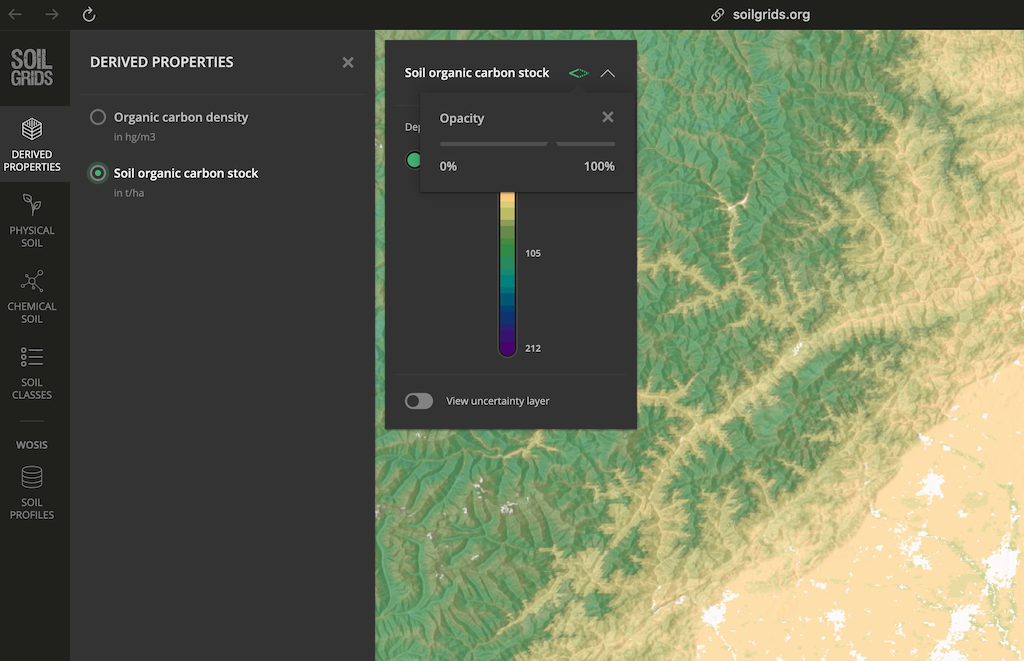
\includegraphics[height=0.75\textheight]{./graphics_david/SoilGrids_SOCstock_Chengdu.png}
\end{figure}
\end{frame}

\begin{frame}{Detail; uncertainty}
\begin{figure}
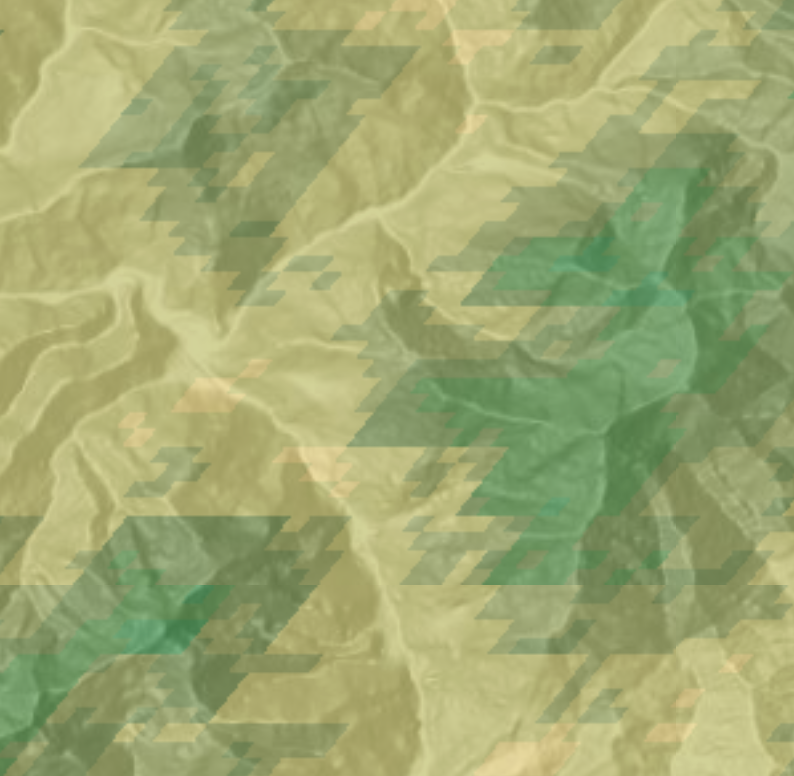
\includegraphics[width=0.4\textwidth]{./graphics_david/SoilGridsDetail.png}
\hfill
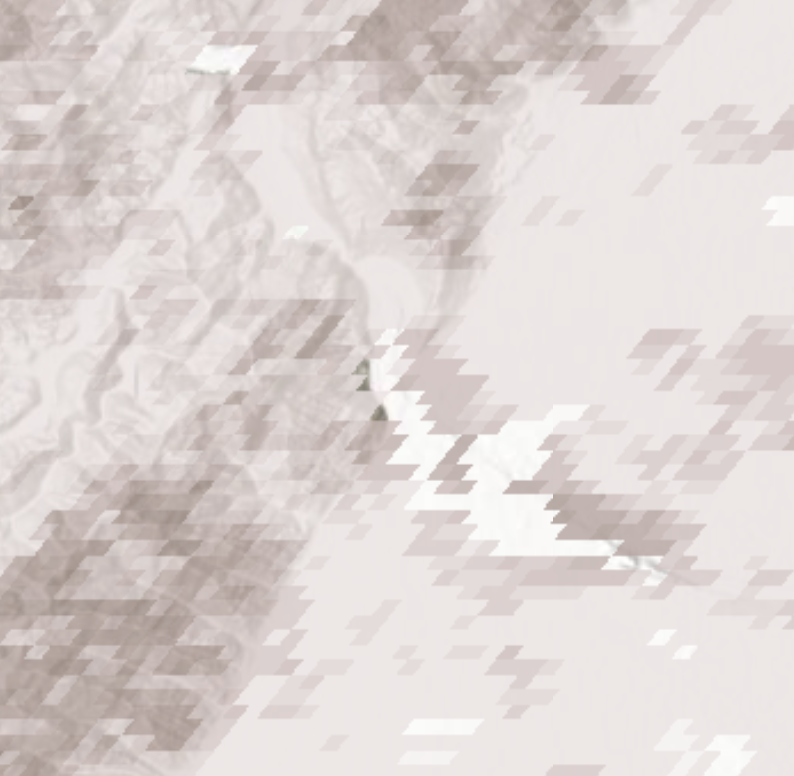
\includegraphics[width=0.4\textwidth]{./graphics_david/SoilGridsUncertainty.png}
\end{figure}
\end{frame}

\begin{frame}
  \frametitle{DSM with disaggregation - 1}
\begin{figure}
  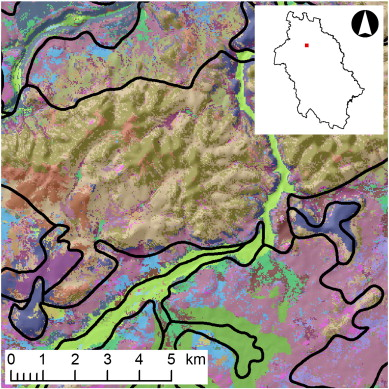
\includegraphics[height=0.55\textheight]{./graphics_david/1-s2.0-S0016706113003522-gr9.jpg}
\end{figure}
Most probable soil class with the original soil polygons overlaid
\\
Source: Odgers \emph{et al.} 2014, \url{doi:10.1016/j.geoderma.2013.09.024}
\end{frame}

\begin{frame}
  \frametitle{DSM with disaggregation - 2}
  \begin{minipage}[b]{0.4\linewidth}
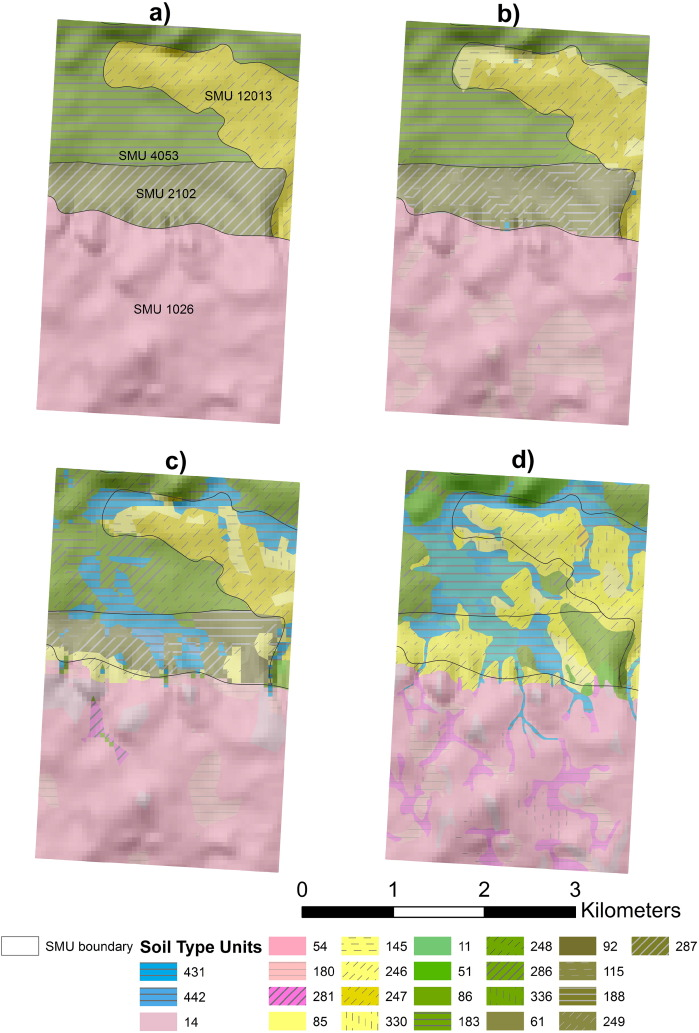
\includegraphics[height=0.75\textheight]{./graphics_david/1-s2.0-S0016706116302464-gr9.jpg}
   \end{minipage}
\hfill
\begin{minipage}[b]{0.58\linewidth}
  a) original 1:250,000 map\\ b) predictive map of Soil Type Units
  without soil-landscape rules for allocating STUs\\c) predictive map
  of Soil Type Units with soil-landscape rules\\d) the observed
  soil map
  \\[1ex]
  Source: Vincent \emph{et al.'} 2018, \url{doi:10.1016/j.geoderma.2016.06.006}
\end{minipage}
\end{frame}

\begin{frame}
  \frametitle{How have these maps been evaluated?}
    \begin{itemize}
        \item On the basis of \textbf{test points}
        \begin{itemize}
            \item independent test set in target area
            \item out-of-bag (OOB) in bagged Machine Learning (ML) methods: members of training set, not used in one calibration
            \item repeated splits into test/training of one dataset
        \end{itemize}
        \item (pointwise) \textbf{evaluation statistics}: ME, RMSE,
          1:1 $R^2$ (MCC, Nash-Sutcliffe Model Efficiency), gain/bias
          of actual regressed on observed \ldots
    \end{itemize}
\end{frame}


\begin{frame}
  \frametitle{Problems with evaluation by point statistics -- Internal}
From the mapper's point of view:
\begin{enumerate}
    \item Based on a \textbf{limited number of observations}, far fewer than the number of predictions (grid cells, ``pixels'').
\item Evaluation points are almost never from an independent \textbf{probability sample}.
\item Cross-validation and data-splitting approaches rely on this \textbf{biased} point set.
\item Evidence: Different DSM approaches can result in maps with quite \textbf{similar "validation statistics" but obviously different spatial patterns}.
  \end{enumerate}
  
\end{frame}


\begin{frame}
  \frametitle{Example of limited evaluation points: ISRIC WoSIS}
\begin{figure}
    \centering
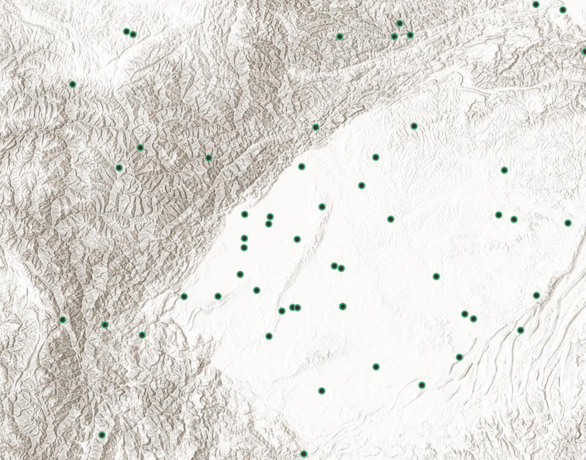
\includegraphics[height=0.7\textheight]{./graphics_david/SoilGridsProfiles_Chengdu.png}
\end{figure}
\end{frame}

\begin{frame}
  \frametitle{Different ML methods, covariates,  points $\to$ different patterns}
    \begin{figure}
        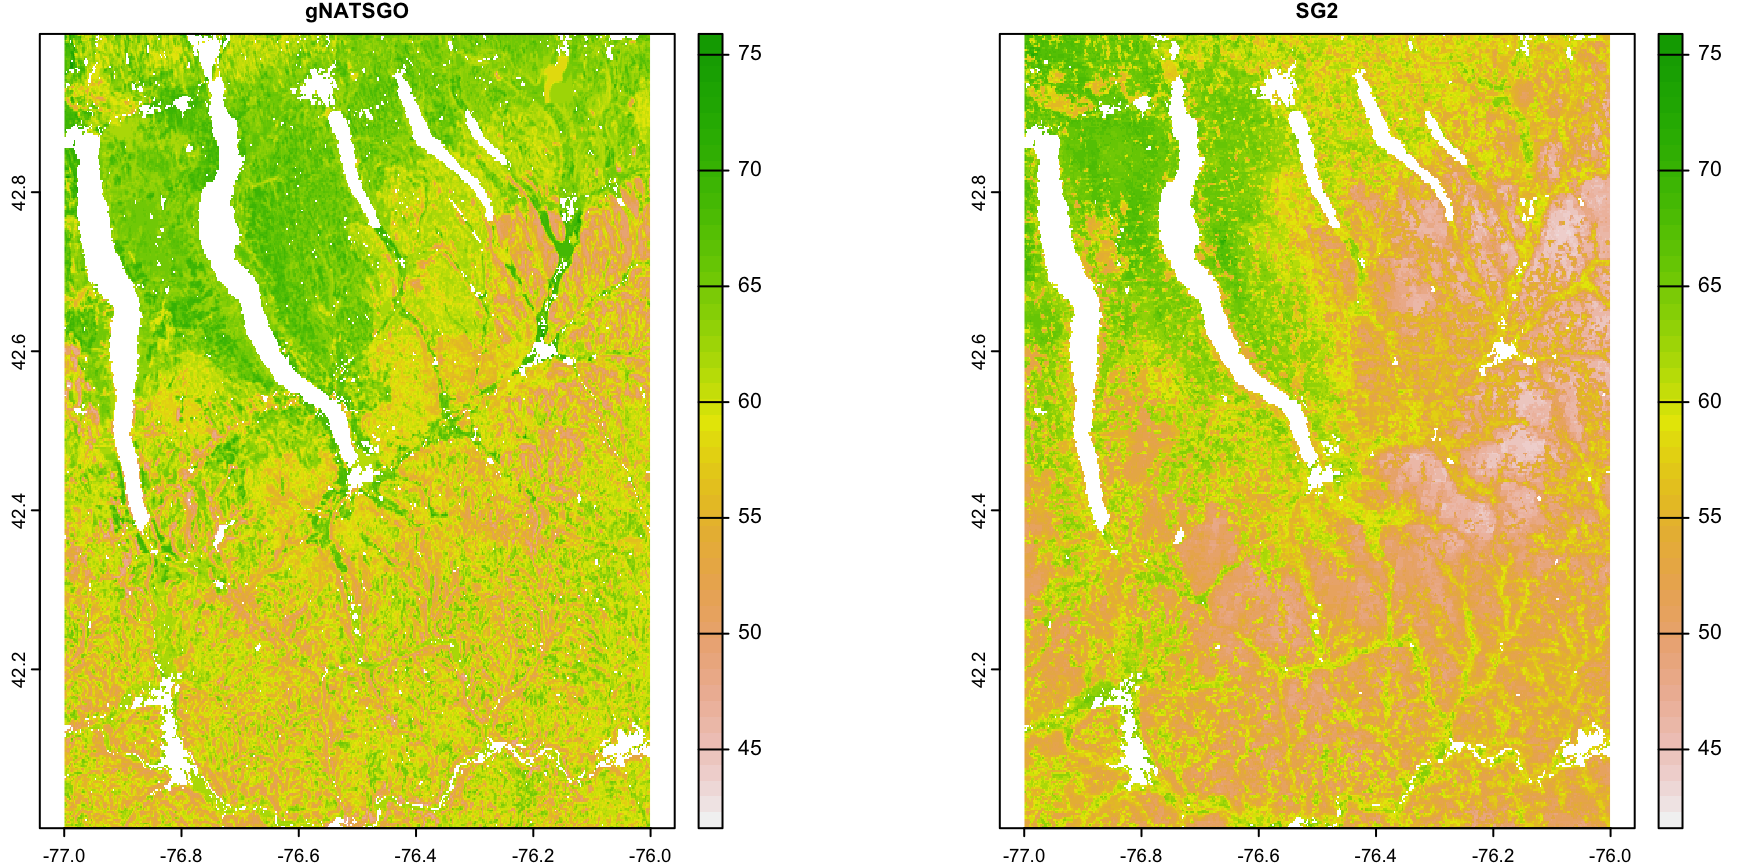
\includegraphics[width=0.49\linewidth]{./graphics_david/Fig07a.png}
        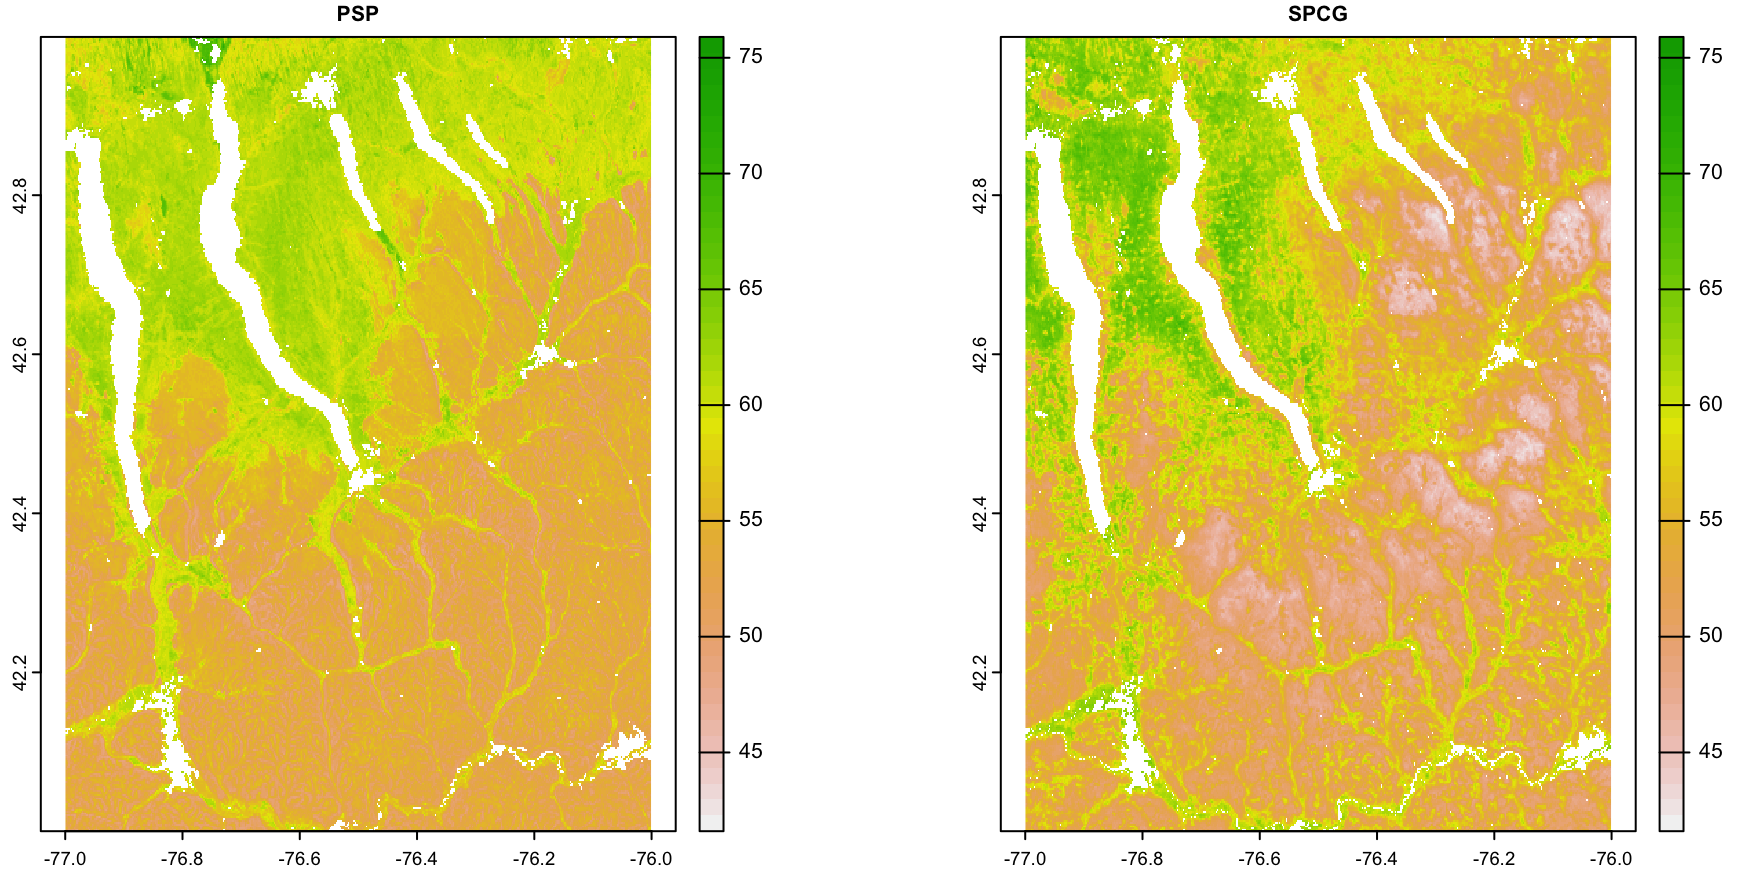
\includegraphics[width=0.49\linewidth]{./graphics_david/Fig07b.png}
\par        
{\hfill        
        {pH x 10, 0-5~cm} \hfill}
    \end{figure}
\end{frame}

\begin{frame}
  \frametitle{Detail}
\begin{figure}
    \centering
    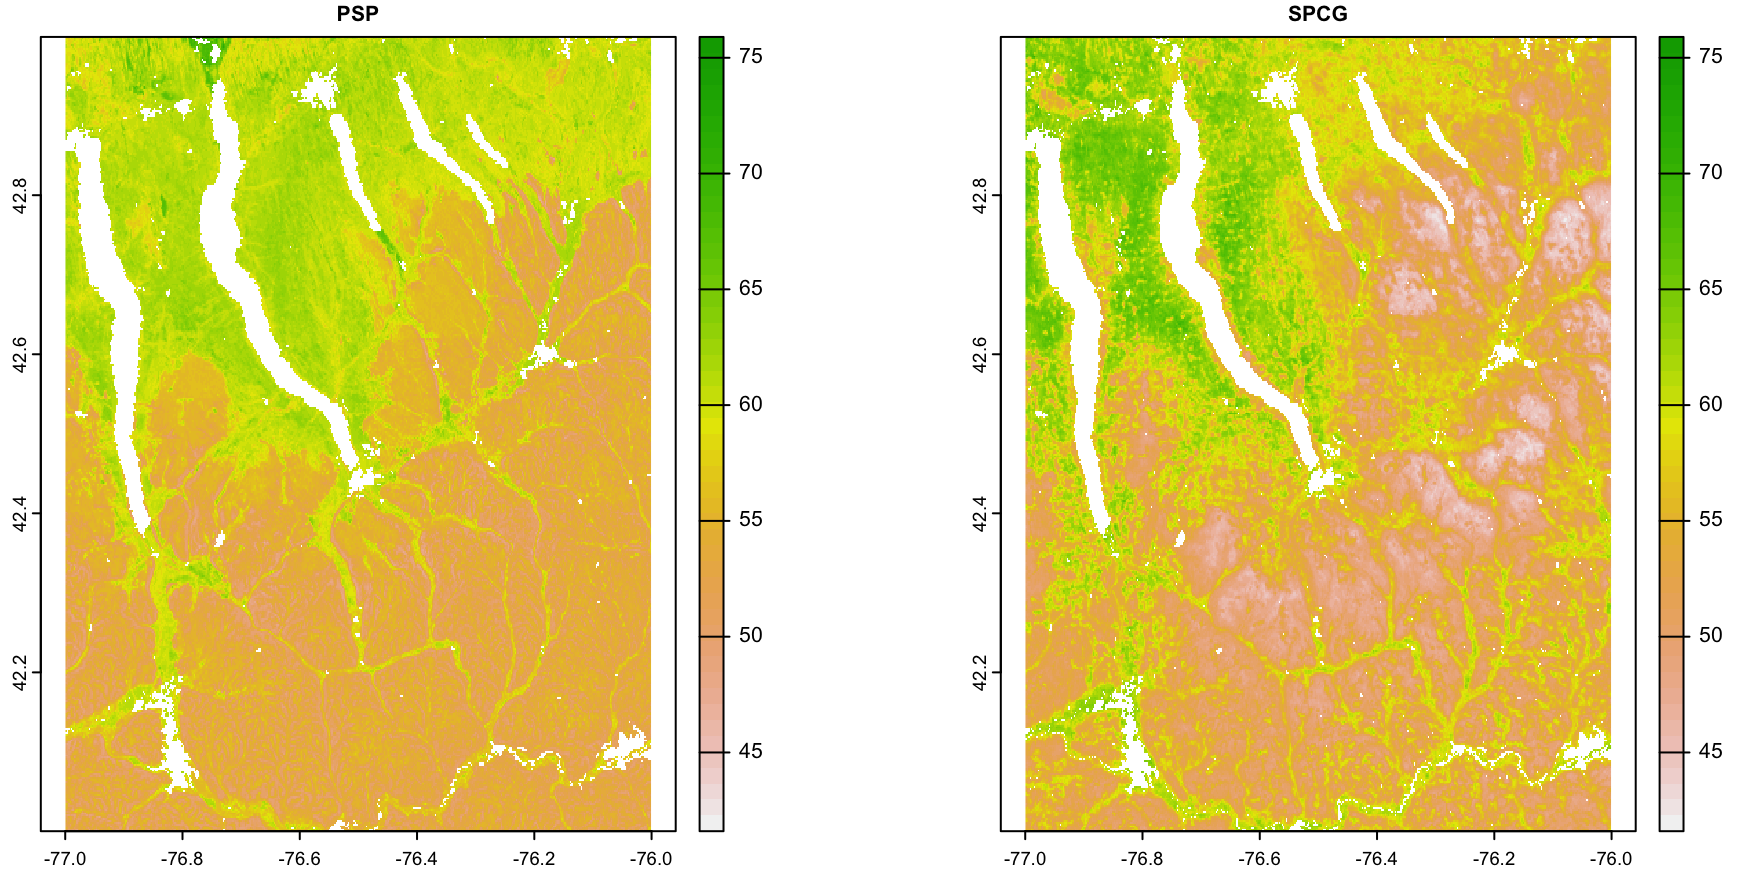
\includegraphics[height=0.72\textheight]{./graphics_david/Fig07b.png}
 \end{figure}
\end{frame}

\begin{frame}
  \frametitle{Different ML methods, covariates,  points $\to$ different patterns}
     \begin{figure}
        \centering
        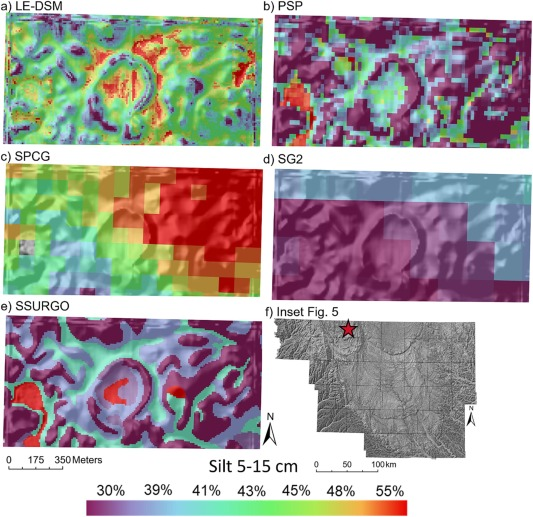
\includegraphics[height=0.7\textheight]{./graphics_david/1-s2.0-S0016706124000107-gr12.jpg}
        \\(Bohn \& Miller 2024)
    \end{figure}
\end{frame}

\begin{frame}
  \frametitle{Different ML methods, covariates,  points $\to$ different patterns}
    \begin{figure}
        \centering
        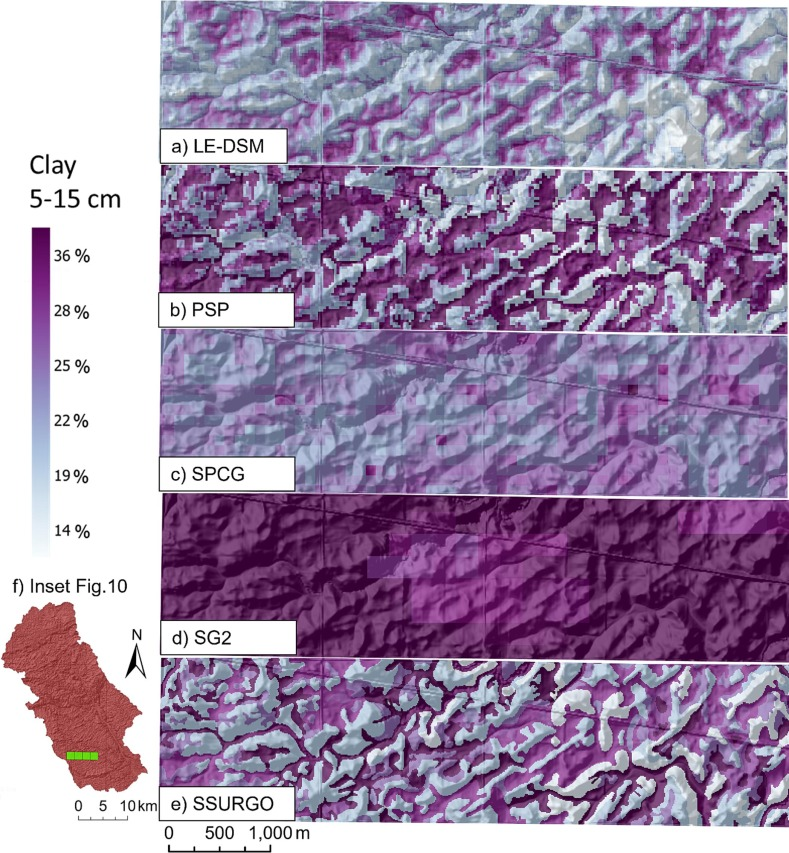
\includegraphics[height=0.7\textheight]{./graphics_david/1-s2.0-S0016706124000107-gr11.jpg}
        \\(Bohn \& Miller 2024)
    \end{figure}
\end{frame}

\begin{frame}
  \frametitle{\textbf{Same} ML method, covariates, points, but different
    \textbf{parameters} $\to$ different patterns}
    \begin{figure}
        \centering
        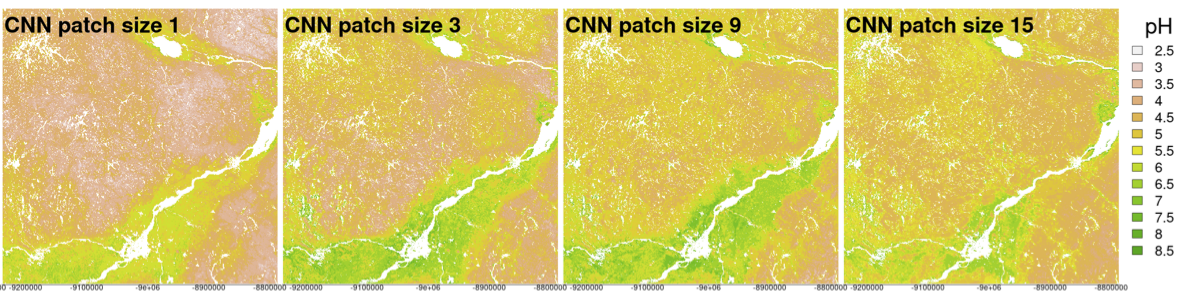
\includegraphics[width=\textwidth]{./graphics_david/GenovaPosterFig1a.png}
        \\{Convolutional Neural Network (CNN), different window size (Giulio Genova, ISRIC)}
    \end{figure}
\end{frame}

\begin{frame}
  \frametitle{But \ldots almost identical evaluation statistics}
    \begin{figure}
        \centering
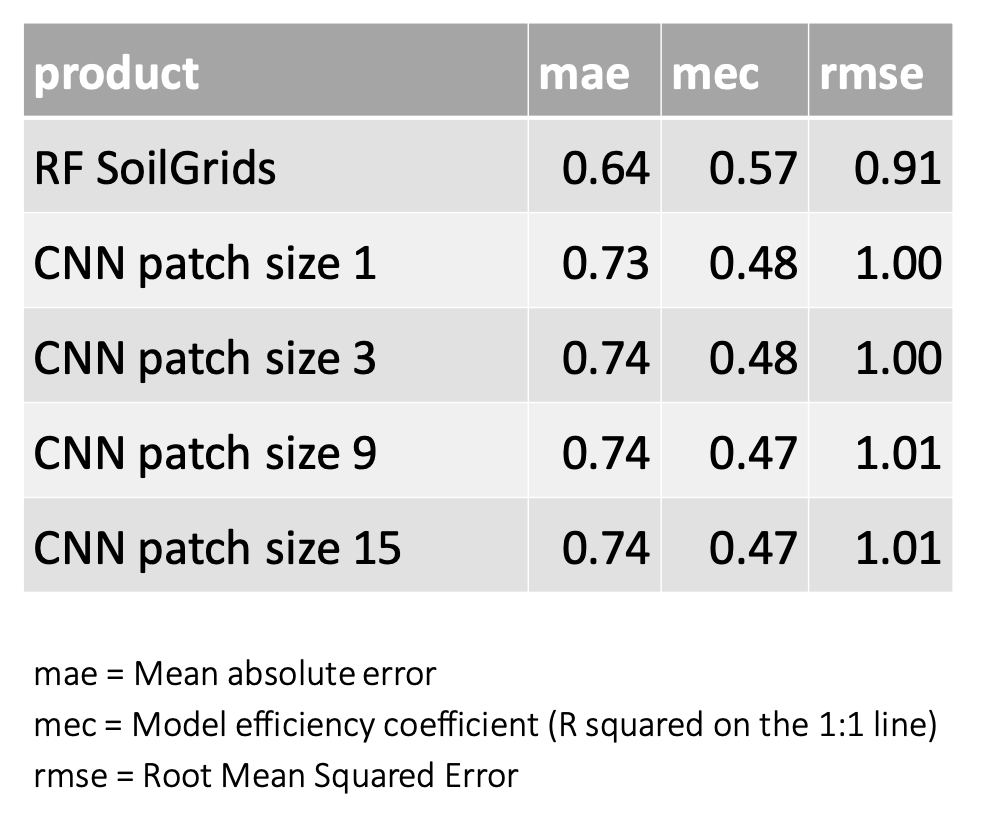
\includegraphics[height=0.7\textheight]{./graphics_david/Genova_poster_stats.png}
     \end{figure}
\end{frame}


\begin{frame}
  \frametitle{Different surveys, different patterns}
    \begin{figure}
        \centering
        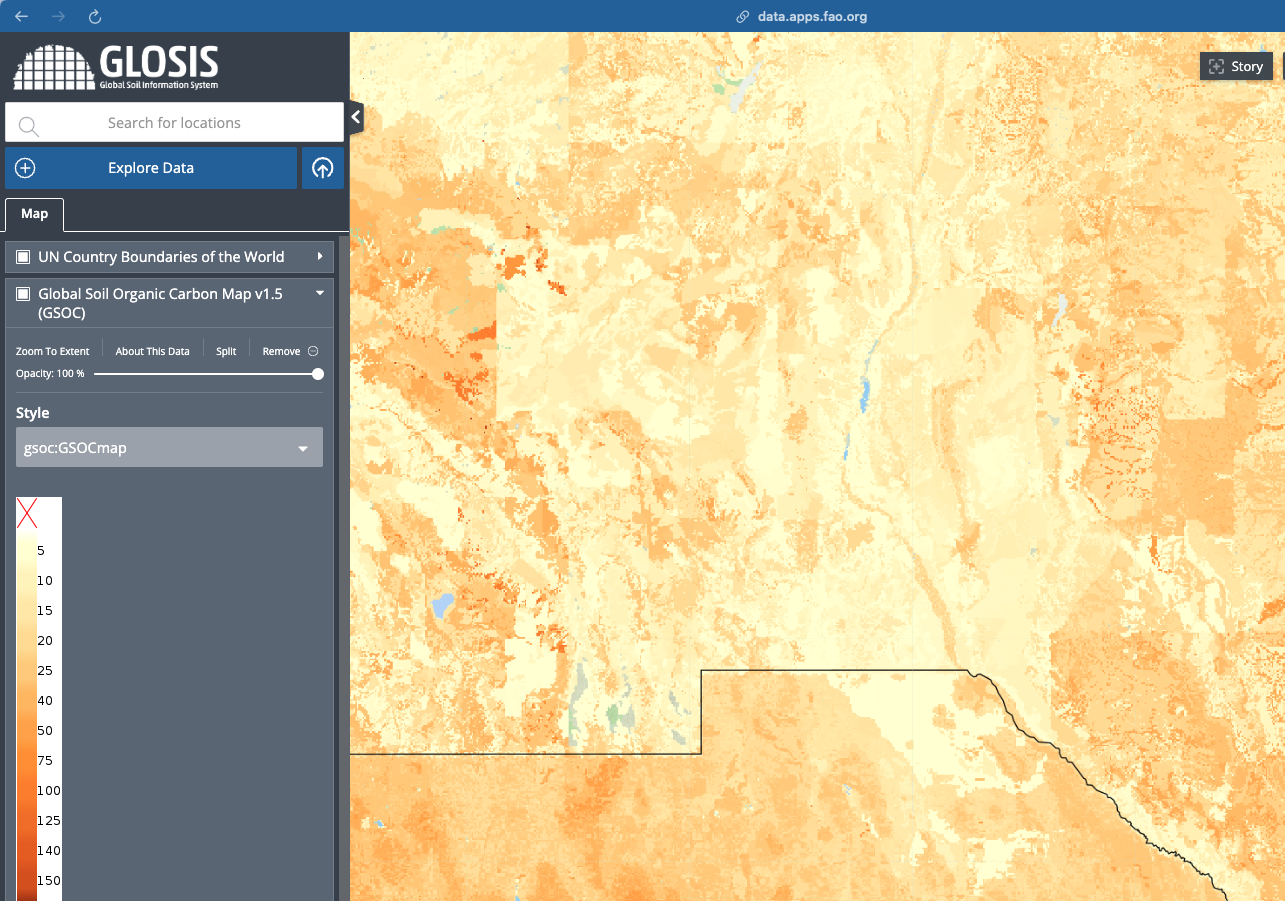
\includegraphics[height=0.8\textheight]{./graphics_david/GLOSIS_SOC_LasCrucesRegion.png}
     \end{figure} 
\end{frame}

\begin{frame}
  \frametitle{Artefacts}
    \begin{figure}
        \centering
        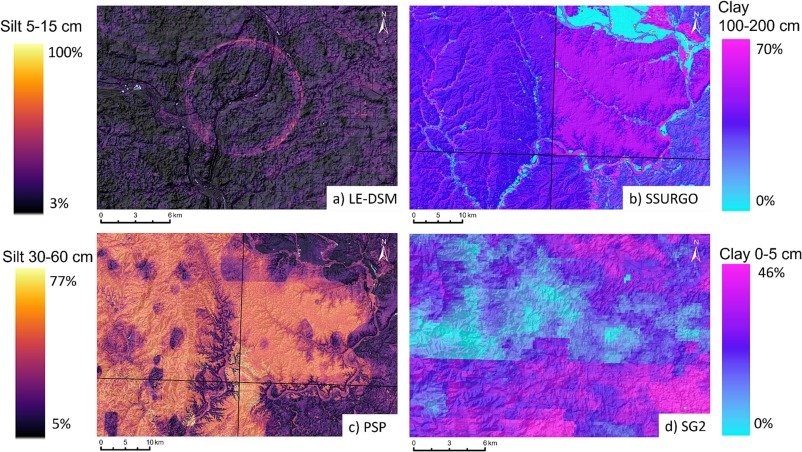
\includegraphics[height=0.7\textheight]{./graphics_david/1-s2.0-S0016706124000107-gr15.jpg}
        \\(Bohn \& Miller 2024)
    \end{figure}
\end{frame}


\begin{frame}{Problems with evaluation by point statistics -- External}

From the map user's point of view:
\begin{enumerate}
\item  Soils are \textbf{managed as units} at some scale, \emph{not} point-wise.
\item  Land-surface models often rely on 2D or 3D \textbf{connectivity} between grid cells.
\item  More than a century of fieldwork has shown that \textbf{soils
    occur in more-or-less homogeneous patches}, \emph{not} as isolated
  pedons (Fridland, Boulaine, Hole \ldots).
\item How to understand and account for \textbf{artefacts}?
  \end{enumerate}
  
\end{frame}

\section{Patterns of soils on the landscape}

\begin{frame}{Scale of patterns of soils on the landscape}
\begin{itemize}
    \item Catena/hillside/toposequence scale
    \begin{itemize}
        \item landscape segments
        \item DSM resolution 50--250~m
        \item mapping scale 1:12k - 1:62.5k
        \item minimum mappable area (MMA) 0.625-10~ha
        \end{itemize}
    \item Detailed scale within segments
    \begin{itemize}
        \item precision agriculture
        \item DSM resolution 1-10~m
        \item mapping scale 1:1k - 1:4k
    \end{itemize}
\end{itemize}
\end{frame}

\begin{frame}{Soil-landscape polygon maps}
\begin{figure}
    \centering    \includegraphics[width=\textwidth]{./graphics_david/pq49b_map_3_part.jpg}
\end{figure}  
\end{frame}

\begin{frame}{Conceptual basis of the soil-landscape model}
    \begin{itemize}
        \item Soilscape segments with different combinations of soil-forming factors
        \item Majority of heterogeneity is \textbf{between} polygons
        \item Identified by a conceptual paradigm (Hudson 1992)
        \item identifiable transitions (but see Lagacherie \textit{et al.} 1996)
        \item \textbf{scale-independent} (??)
    \end{itemize}
\end{frame}

\begin{frame}{Soilscape segments, 1:12k -- 1:24k}
    \begin{figure}
        \centering
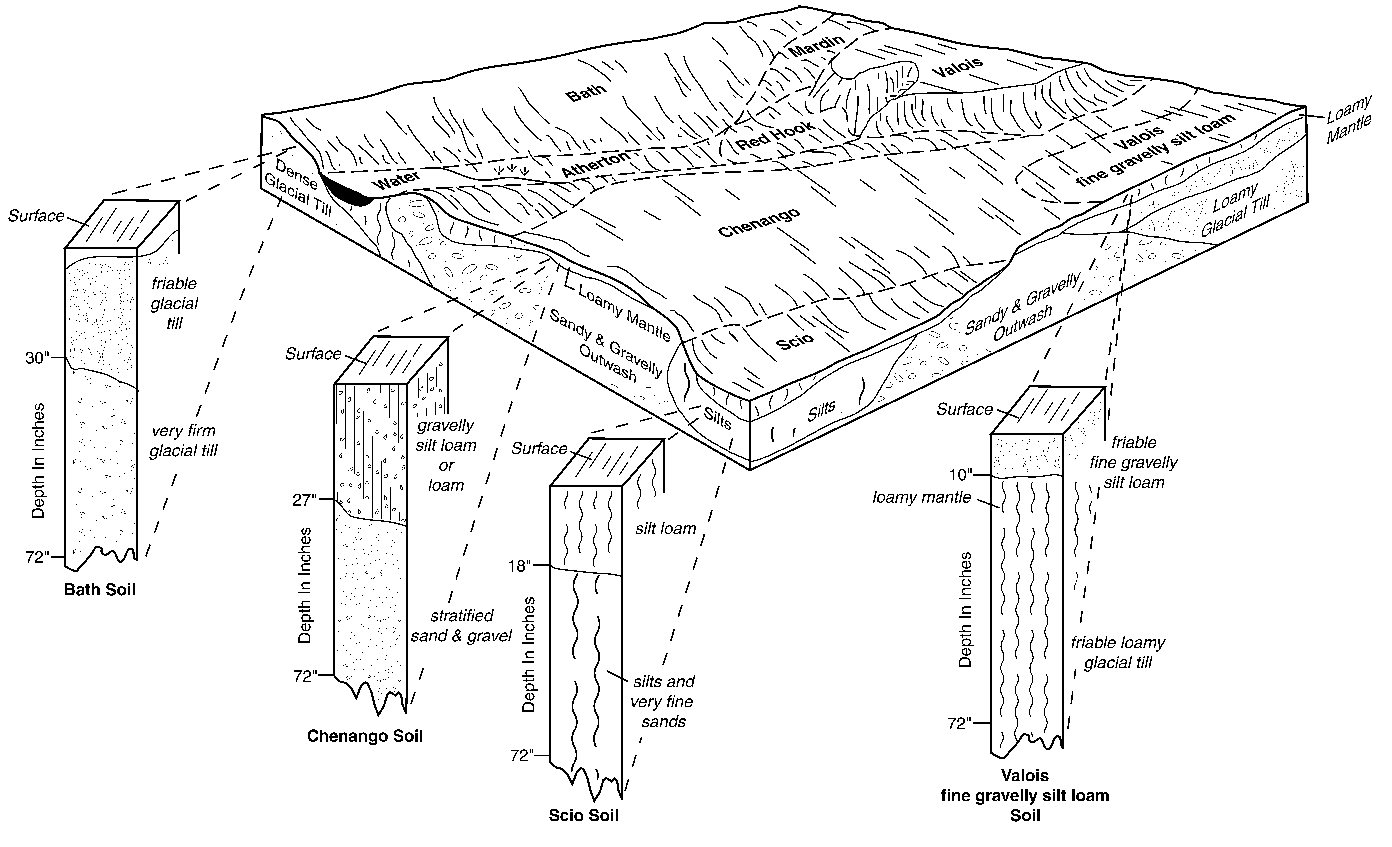
\includegraphics[height=0.65\textheight]{./graphics_david/NY-2010-09-28-14.pdf}\\
{Conceptual block diagram, Otsego County NY (USA)}
     \end{figure}
\end{frame}

\begin{frame}{Detailed (1:24k) soil survey: pattern of landscape segments}
    \begin{figure}
        \centering
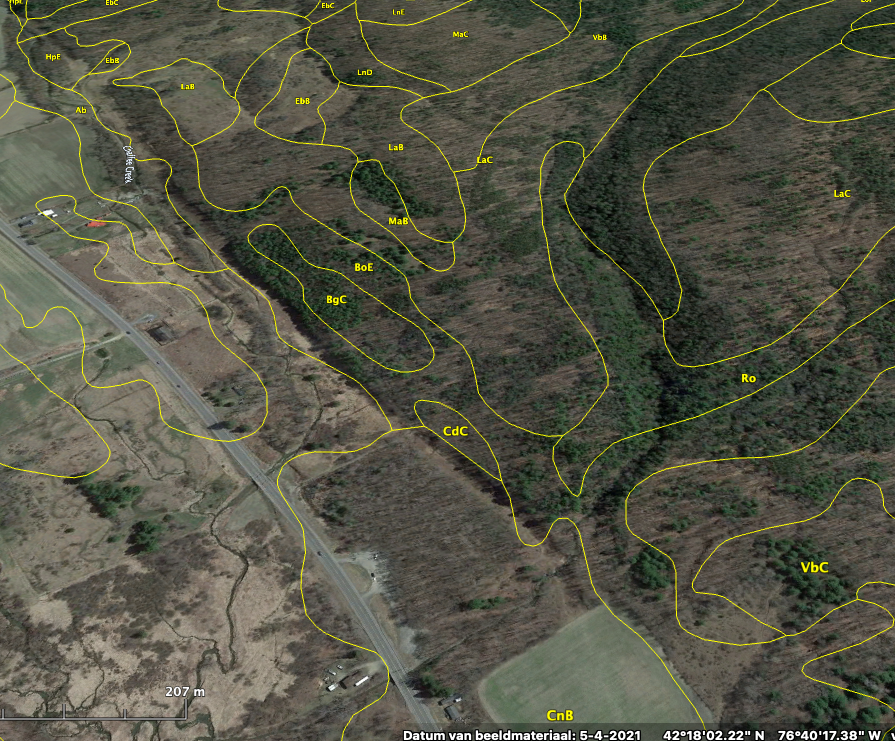
\includegraphics[height=0.7\textheight]{./graphics_david/PonyHollow_SoilWeb_Screenshot_relief.png}\\
{\footnotesize centre -76\textdegree 40'23" E, 42\textdegree 18'10" N}
     \end{figure}
    \end{frame}

\begin{frame}{Map unit components}
    \begin{figure}
        \centering
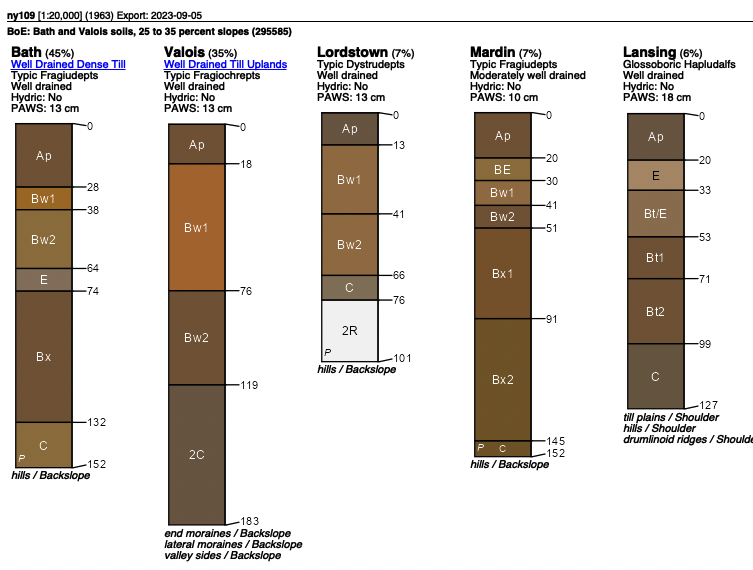
\includegraphics[height=0.75\textheight]{./graphics_david/Bath_Valois_profiles.png}
     \end{figure}
    \end{frame}

\begin{frame}{Field-level patterns, 1:1k -- 1:4k}
        \begin{figure}
        \centering
\includegraphics[height=0.65\textheight]{./graphics_david/WoodCoOH_Hoytville_cl_detail.png}\\
{Wood County, Ohio (USA); \texttt{HoA}: Hoytville clay loam}
     \end{figure}
\end{frame}

\begin{frame}{Same soilscape at different resolution}
    \begin{figure}
        \centering
        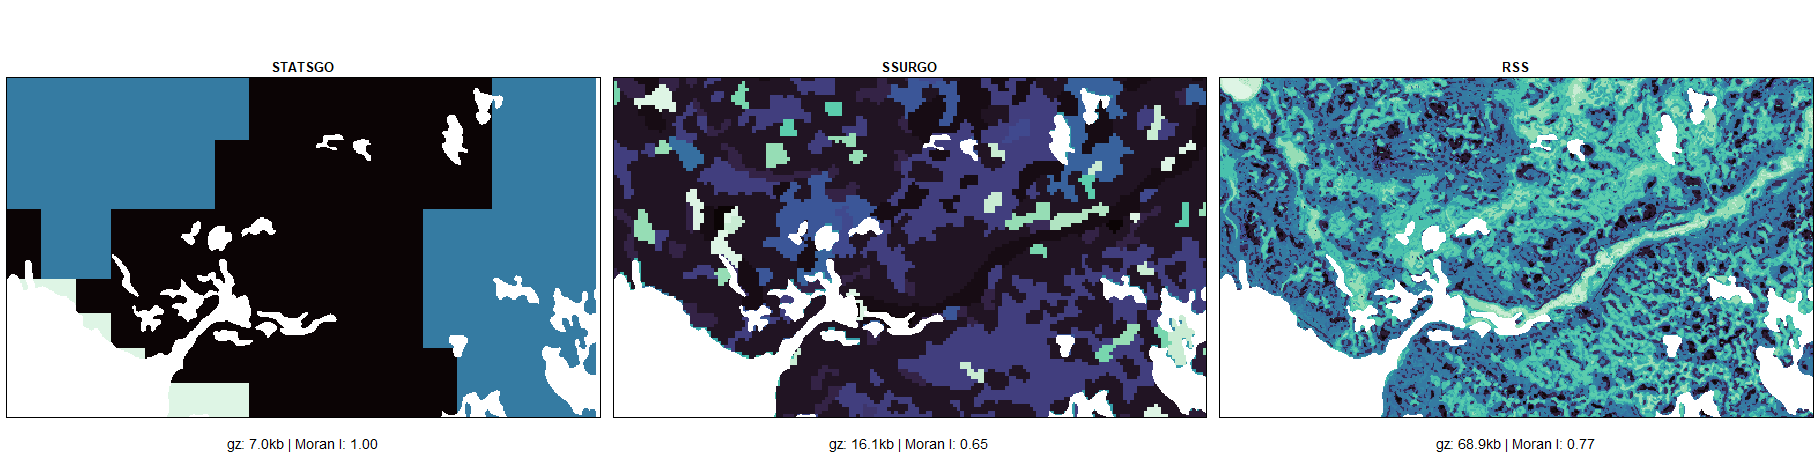
\includegraphics[width=\linewidth]{./graphics_david/Dylan_ND005-example-01.png}
\\source: Dylan Beaudette (NRCS)
    \end{figure}
\end{frame}

\begin{frame}{Are there mathematically ``natural'' soil patterns?}
\begin{itemize}
    \item Neutral Landscape Models (Riitters et al. 2007, 2009) for landscape ecology
    \begin{itemize}
        \item Attempt to reproduce landscape patterns (e.g., vegetation patches) with mathematical models
        \item \textbf{Do soils also occur in these patterns?}
    \end{itemize}
    \item \texttt{NLMR}, \texttt{landscapetools} R packages (Sciani 2018)
\end{itemize}
\end{frame}

\begin{frame}{Neutral landscapes}
        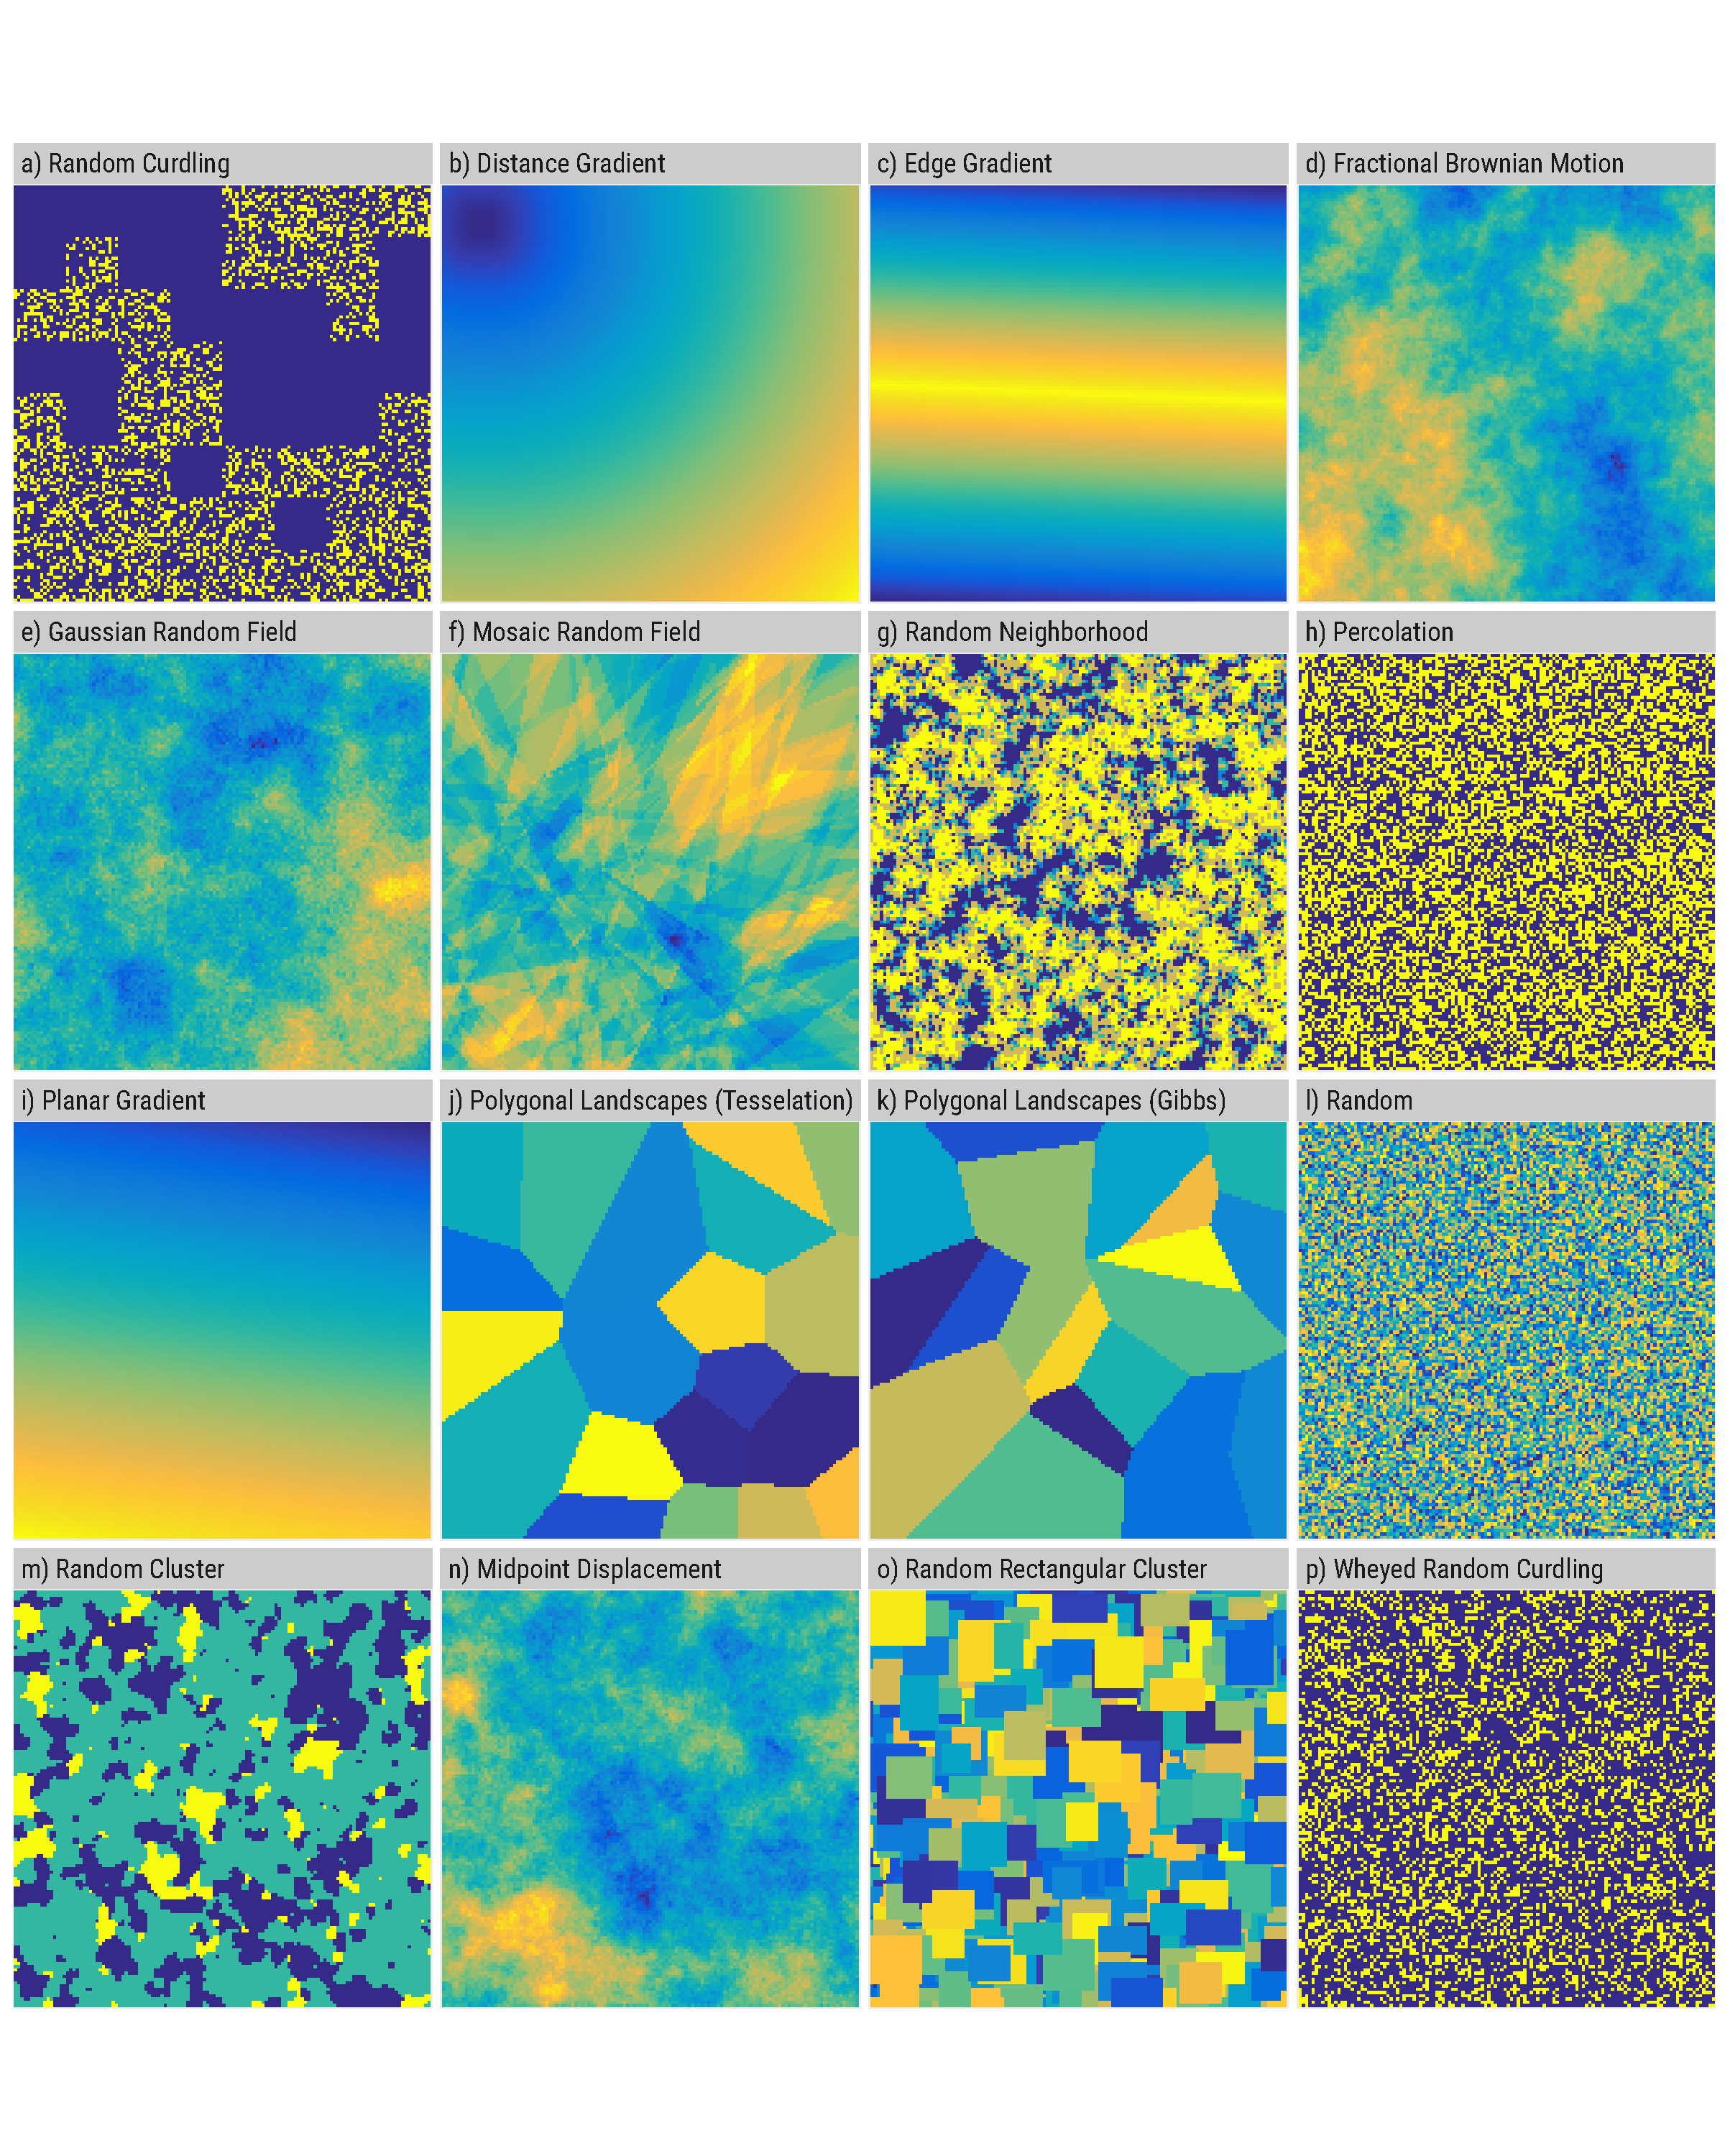
\includegraphics[height=0.65
        \textheight]{graphics_david/marcosci-Sciaini_et_al_2018-e3aa0ce_bestiary.pdf}
\\source: Sciaini et al. (2018)
    \hfill
    Which ``look like'' soil patterns?
\end{frame}

\section{Pattern analysis}

\begin{frame}{Pattern analysis}
    \begin{itemize}
        \item Quantitative description of (spatial) patterns
        \item Long history in image analysis
        \item Applied to landscape mosaics (FRAGSTATS)
        \item R packages  \texttt{motif}, \texttt{landscapemetrics}, \texttt{rassta} \ldots
        \item Stand-alone \texttt{geoPat}\footnote{\url{https://github.com/Nowosad/geopat2}}
\begin{quote}
\scriptsize
    ``GeoPAT’s core idea is to tessellate global spatial data into grid of square blocks of original cells (pixels). This transforms data from its original form (huge number of cells each having simple content) to a new form (much smaller number of supercells/blocks with complex content)''
\end{quote}
   \end{itemize}
\end{frame}

\begin{frame}{Levels of pattern analysis}
\begin{enumerate}
    \item Characterize the pattern of one map
    \item Compare patterns of several maps
    \item Evaluate pattern with respect to ``reality''
    \item Segment map by its patterns
\end{enumerate}
\vspace{2ex}
Different methods for \textbf{continuous} and \textbf{classified} maps
\end{frame}

\subsection{Continuous soil properties maps}

\begin{frame}{Characterizing patterns -- continuous soil properties}
    \begin{enumerate}
        \item Local variogram analysis: spatial scale of finest resolution
        \item Moving-window autocorrelation: how does this vary across the DSM?
    \end{enumerate}
\end{frame}

\begin{frame}{Variograms with fitted models}
    \begin{figure}
        \centering
        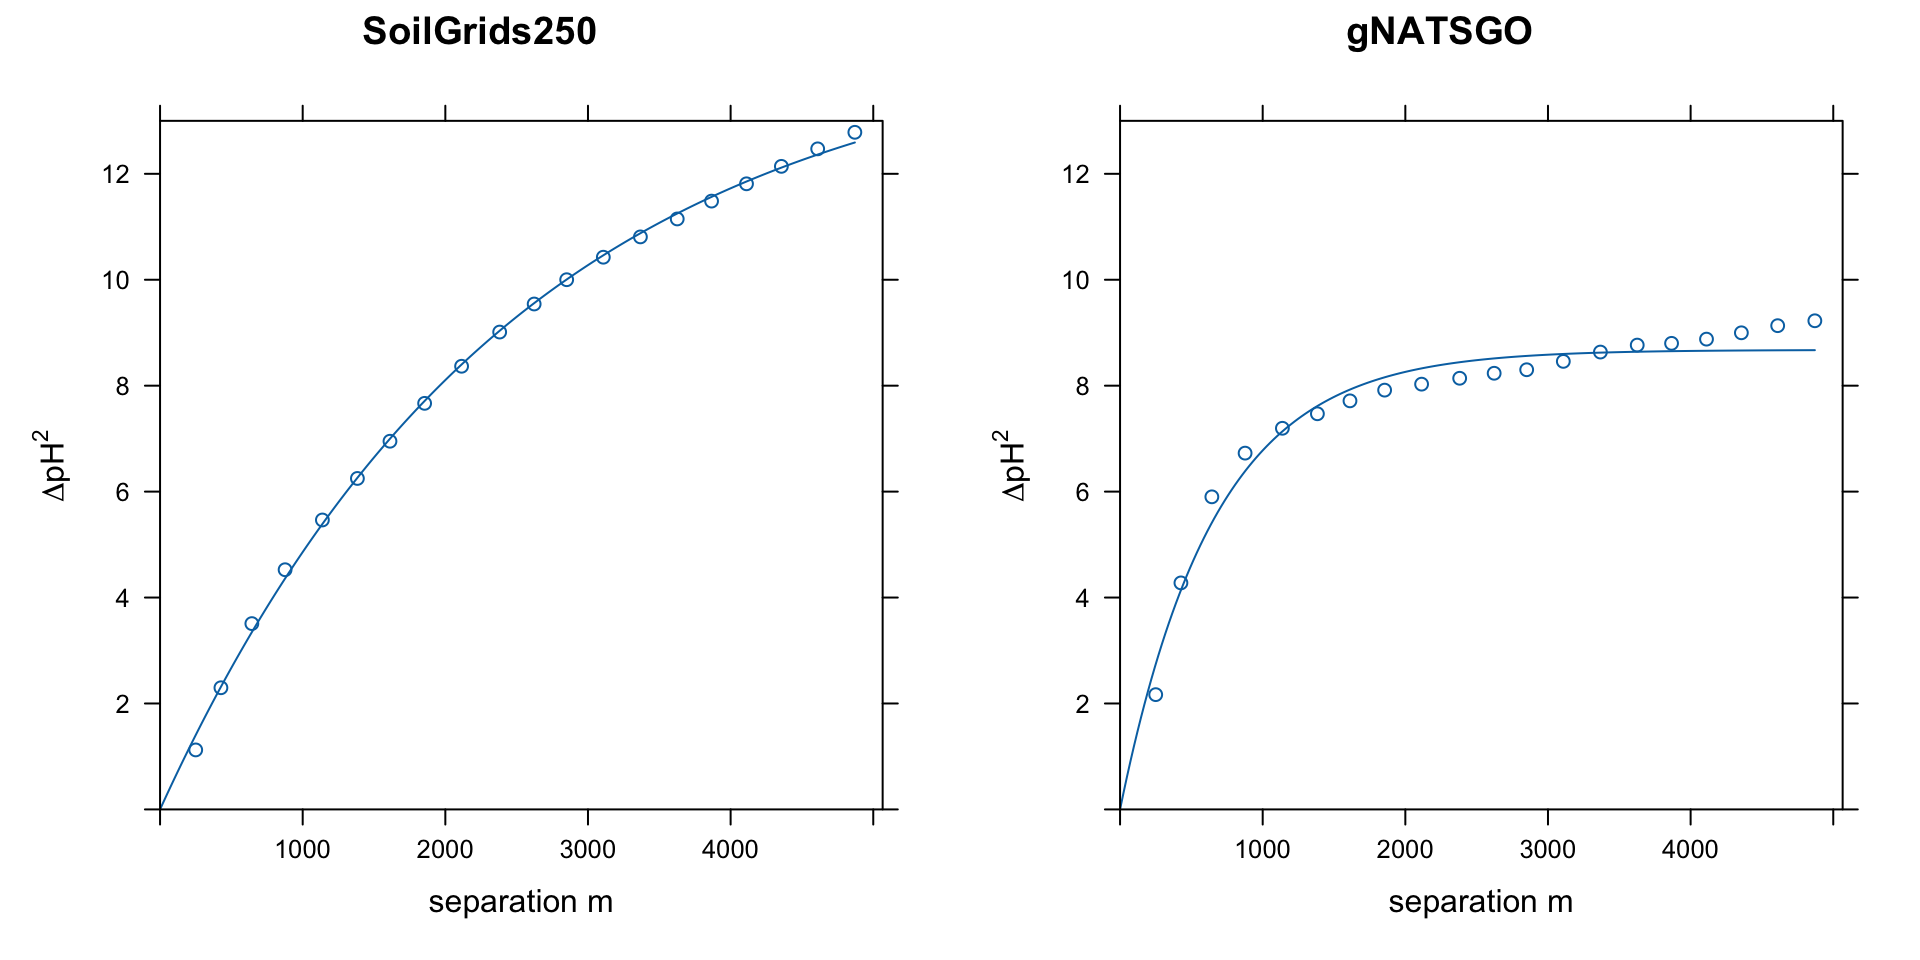
\includegraphics[height=0.6\textheight]{./graphics_david/variograms.png}
\\${(\mathrm{pH} * 10)}^2$; interpret sill and range
    \end{figure}
\end{frame}

\begin{frame}{Comparing local spatial structure with fitted variogram parameters}

% latex table generated in R 4.2.1 by xtable 1.8-4 package
% 
\begin{tabular}{lrrr}
  \hline
Product & Effective range & Structural Sill & Proportional Nugget \\ 
  \hline
gNATSGO & 1938.00 & 10.32 & 0.00 \\ 
  SG2 & 3699.00 & 12.93 & 0.00 \\ 
  SPCG & 6924.00 & 11.81 & 0.01 \\ 
  PSP & 3918.00 & 6.50 & 0.02 \\ 
   \hline
\end{tabular}


\par
Fitted variogram parameters, pH 0-5~cm.
\\
Effective range in m; structural sill in $(\mathrm{pH}x10)^2$, proportional nugget on $[0 \ldots 1]$    
\end{frame}

\begin{frame}{Moving-window autocorrelation}
    \begin{figure}
        \centering
        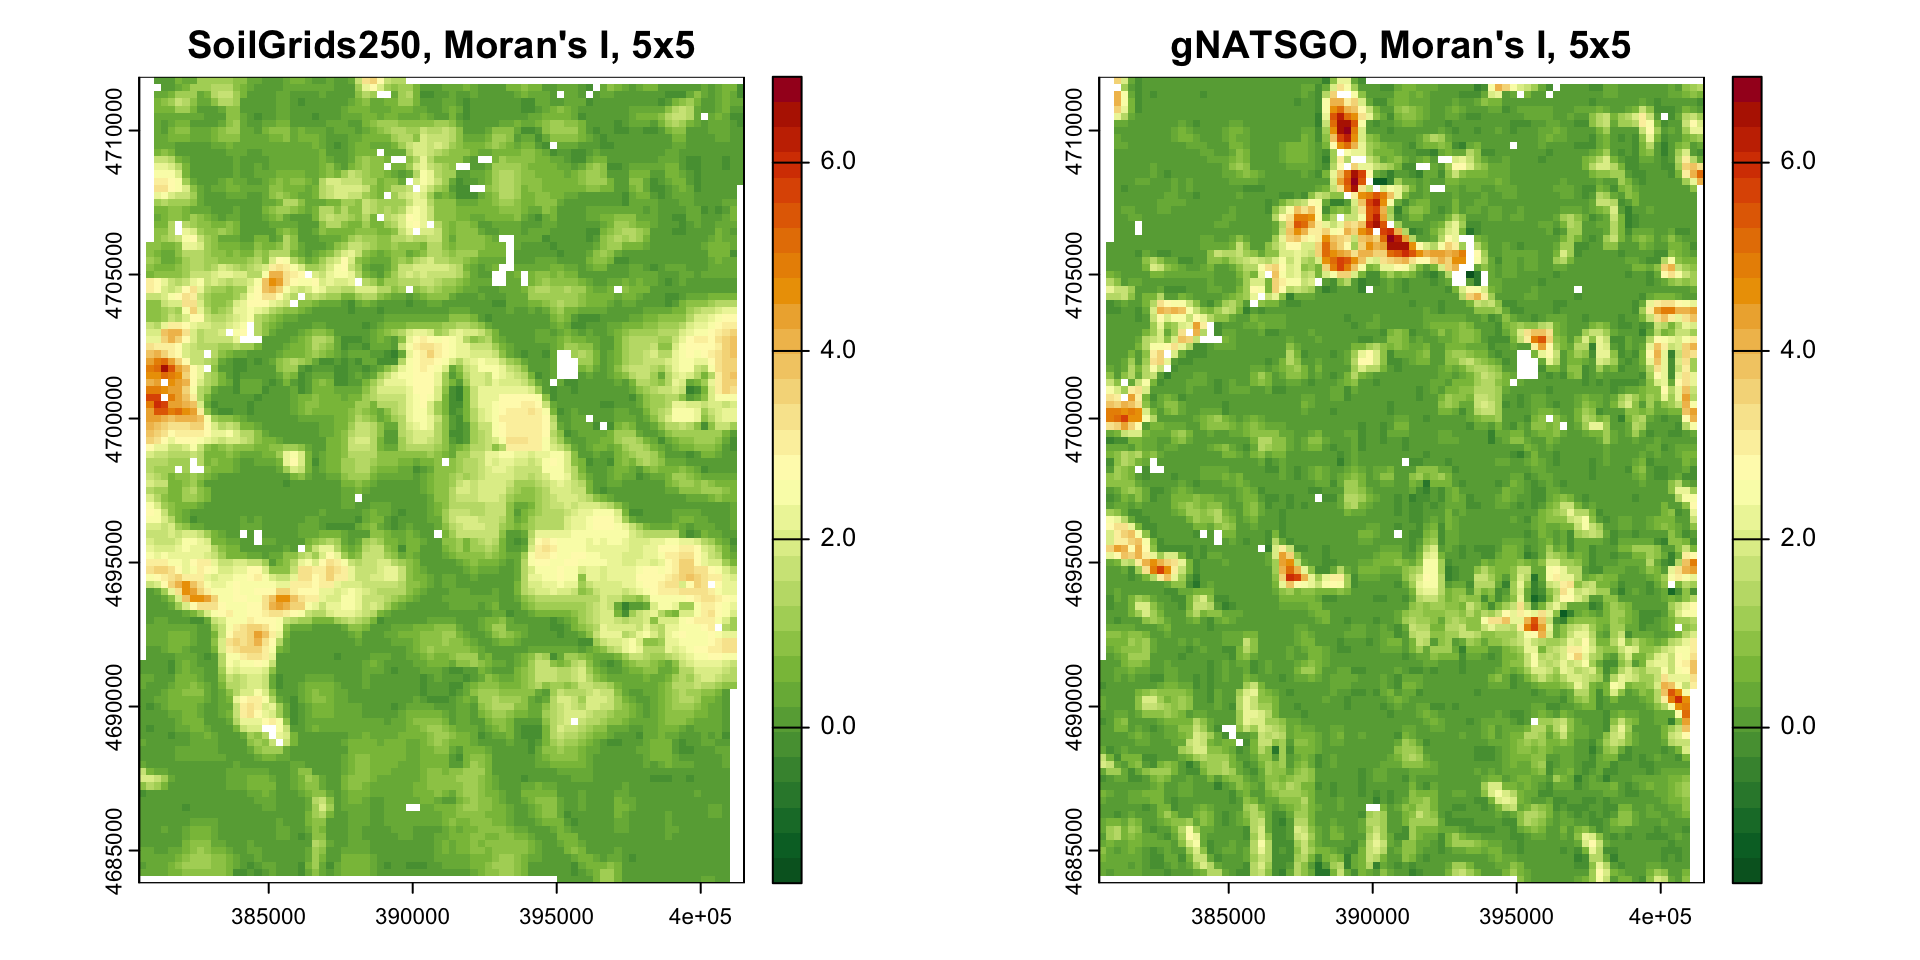
\includegraphics[height=0.7\textheight]{./graphics_david/moving-window-5-1.png}
        \\global Moran's $I$ 1.02 (SG250), 0.68 (gNATSGO)
    \end{figure}
\end{frame}

\begin{frame}{Difference map of continuous property -- this also has a pattern}
        \centering        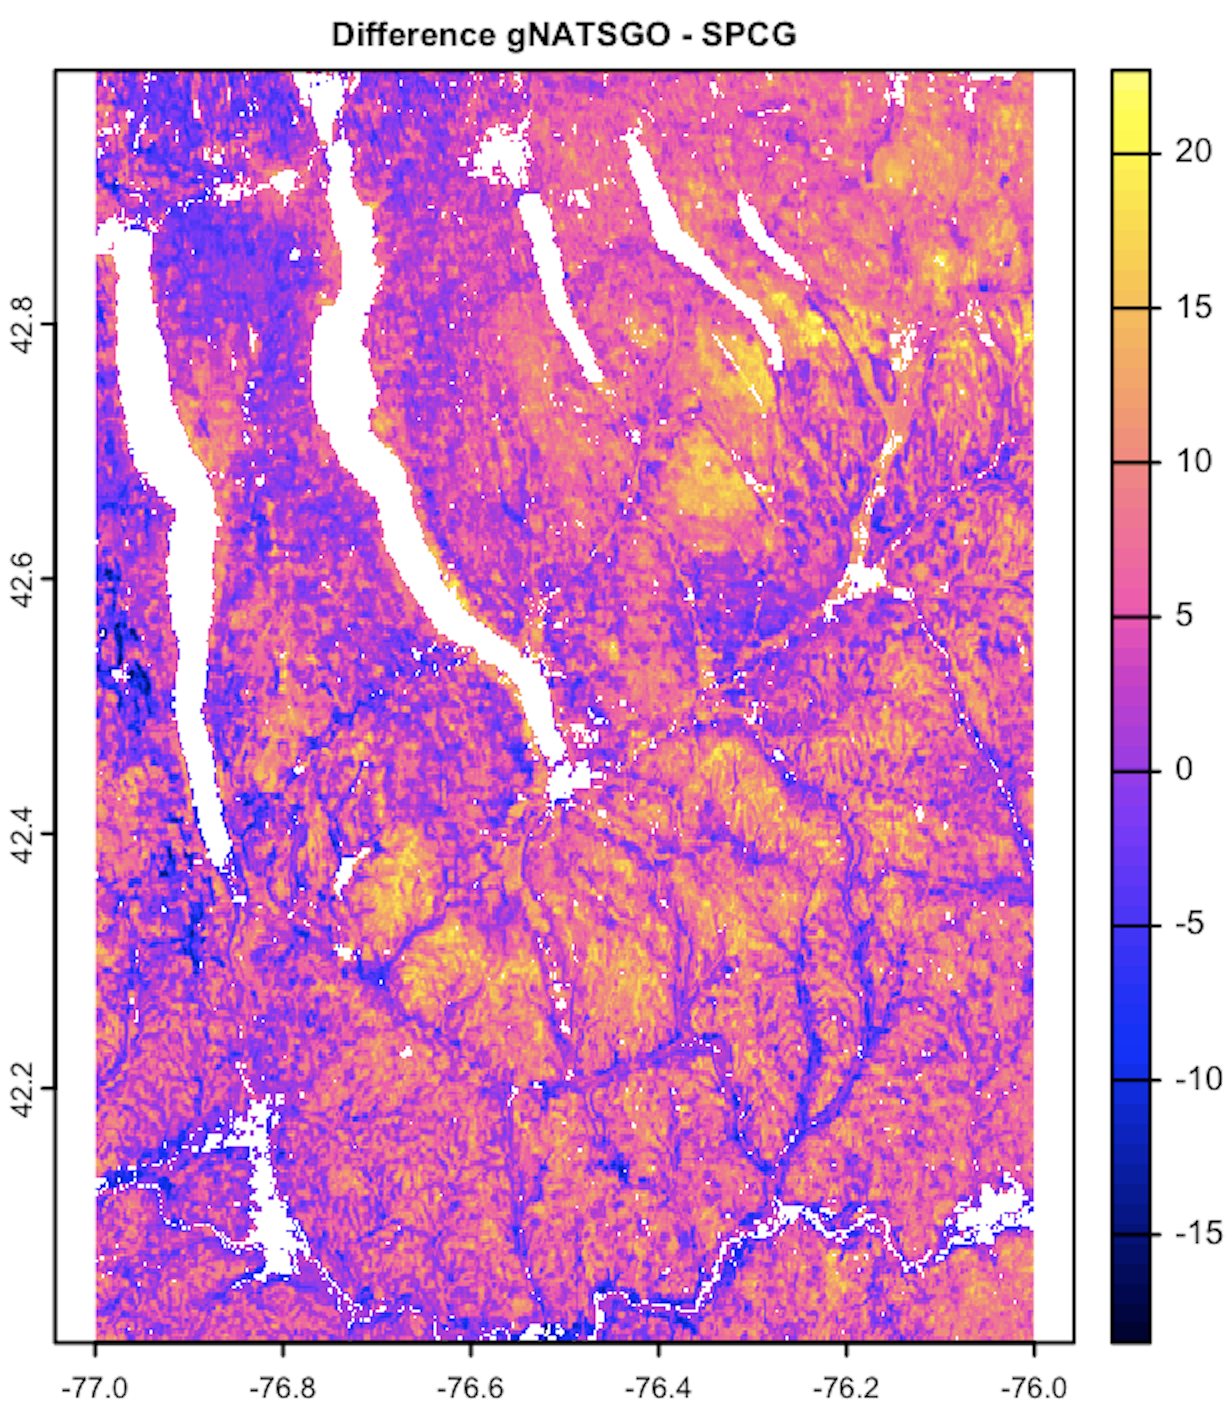
\includegraphics[height=0.72\textheight]  {graphics_david/Delta_gNATSGO_SG_ph05.png}
\\
$\Delta \mathrm{pH x 10}$
\end{frame}


\subsection{Class maps}

\begin{frame}{Characterizing patterns -- classified soil properties or soil classes}
\begin{itemize}
    \item Well-known techniques from landscape ecology (FRAGSTATS)
    \item Select metrics that are relevant to the objective
    \begin{itemize}
        \item here, characterizing the soil pattern
    \end{itemize}
    \item For continuous properties must \textbf{slice} (discretize)
    \begin{itemize}
        \item meaningful limits, or \ldots
        \item equal-intervals, or \ldots
        \item histogram equalization
    \end{itemize}
\end{itemize}
\end{frame}

\begin{frame}{Histogram equalization in 8 classes}
    \begin{figure}
        \centering
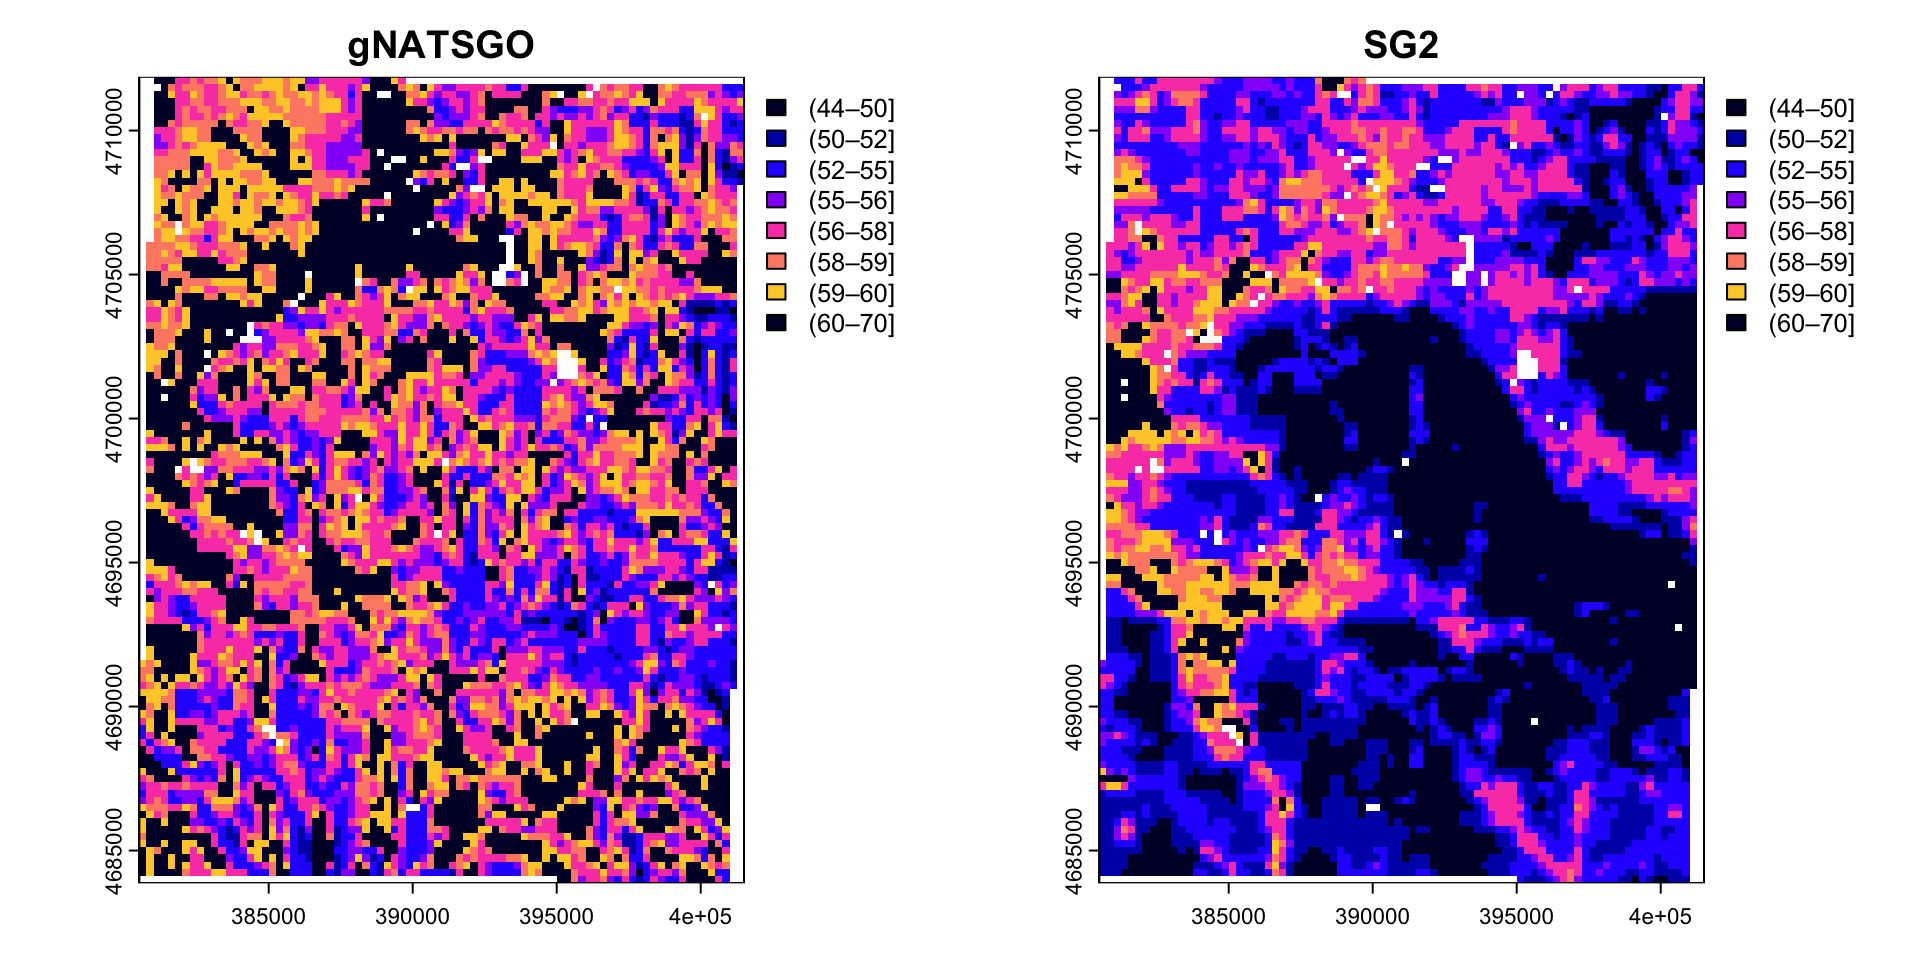
\includegraphics[height=0.8\textheight]{graphics_david/show.classified-1.png}
    \end{figure}
\end{frame}

\begin{frame}{Some relevant metrics}
\begin{itemize}
    \item landscape aggregation index \texttt{LAI}
    \item mean fractal dimension \texttt{MFD}
    \item landscape shape index \texttt{LSI}
    \item Shannon diversity index \texttt{SHDI}
    \item Shannon evenness index \texttt{SHEI}
    \item Co-occurrence vector \texttt{COVE}
\end{itemize}    
\end{frame}

\begin{frame}{Metric: landscape aggregation index}

This quantifies how \textbf{connected} is each class, averaged over all classes.
    $$\mathrm{LAI} = \Bigg[∑_{i=1}^m \Big( \frac{g_{ii}}{max-g_{ii}} \Big) P_{i} \Bigg](100)$$
    
    where $g_{ii}$ is the number of like adjacencies, $(\mathrm{max}-g_{ii})$ is the classwise maximum possible number of like adjacencies of class $i$
\par
    Low values: classes are scattered over the map; high values: classes tend to clump together
\end{frame}

\begin{frame}{Metric: mean fractal dimension}

A shape metric, describing multi-scale patch complexity.
$$\mathrm{FRAC} = \frac{2 * \ln * (0.25 * p_{ij})} {\ln a_{ij}}$$ 

where the patch perimeters are ${p_{ij}}$ in linear units and the areas are ${a_{ij}}$ in square units.

\end{frame}

\begin{frame}{Metric: landscape shape index}
    This quantifies the \textbf{complexity of the patch shapes}, across the map.
    $$   \mathrm{LSI} = \frac{0.25 E'}{\sqrt{A}}$$

    where $A$ is the total area of the landscape and $E'$ is the total length of edges, including the boundary.
\end{frame}

\begin{frame}{Metric: Shannon diversity index}
    This measures both the number of classes and their relative abundance. It is a measure of (1) the \textbf{legend complexity}, (2) the \textbf{(un)balance} between classes.
    $$ D = - \sum_{i=1}^N p_i \ln p_i$$

    where $p_i$ is the proportion of pixels of class $i = (1 \ldots N)$
\end{frame}

\begin{frame}{Comparing maps with these metrics}
\par
    % latex table generated in R 4.2.1 by xtable 1.8-4 package
% 
\begin{tabular}{llllll}
  \hline
product & ai & frac\_mn & lsi & shdi & shei \\ 
  \hline
gNATSGO & 48.188 & 1.034 & 22.602 & 1.666 & 0.801 \\ 
  SG2 & 50.659 & 1.034 & 21.768 & 2.06 & 0.991 \\ 
  SPCG & 58.483 & 1.041 & 18.557 & 1.887 & 0.907 \\ 
  PSP & 47.025 & 1.04 & 23.232 & 1.898 & 0.913 \\ 
   \hline
\end{tabular}

    \par
    Landscape metrics statistics, pH 0--5~cm (top); 30--60~cm (bottom). \texttt{frac\_mn}: Mean Fractal Dimension; \texttt{lsi}: Landscape Shape Index; \texttt{shdi}: Shannon Diversity; \texttt{shei}: Shannon Evenness; \texttt{ai}: Aggregation Index\\
    (Longitude -77---76\textdegree, Latitude 42--43\textdegree)
\end{frame}

\begin{frame}{V-measure (Nowosad \& Stepinski 2018)}
\begin{itemize}
    \item Compares \textbf{different spatial partitions} into classes
\item Two maps could have the same \textbf{total areas} of each class, and even the same \textbf{number of polygons} within each class, and even the same \textbf{size distribution} of these polygons \ldots
\item \ldots and yet be completely different in \textbf{how they partition space} into classes.
\item \textbf{homogeneity}: variance of the regions within a zone, normalized by the variance of the regions in the entire domain of the \textbf{first} map
\item \textbf{completeness}: variance of the zones within a region, normalized by the variance of the zones in the entire domain of the \textbf{second} map.
\item $V = \frac{h \times c}{h + c}$
\end{itemize}
\end{frame}

\begin{frame}{Comparing two maps with V-measures}
    \begin{figure}
        \centering        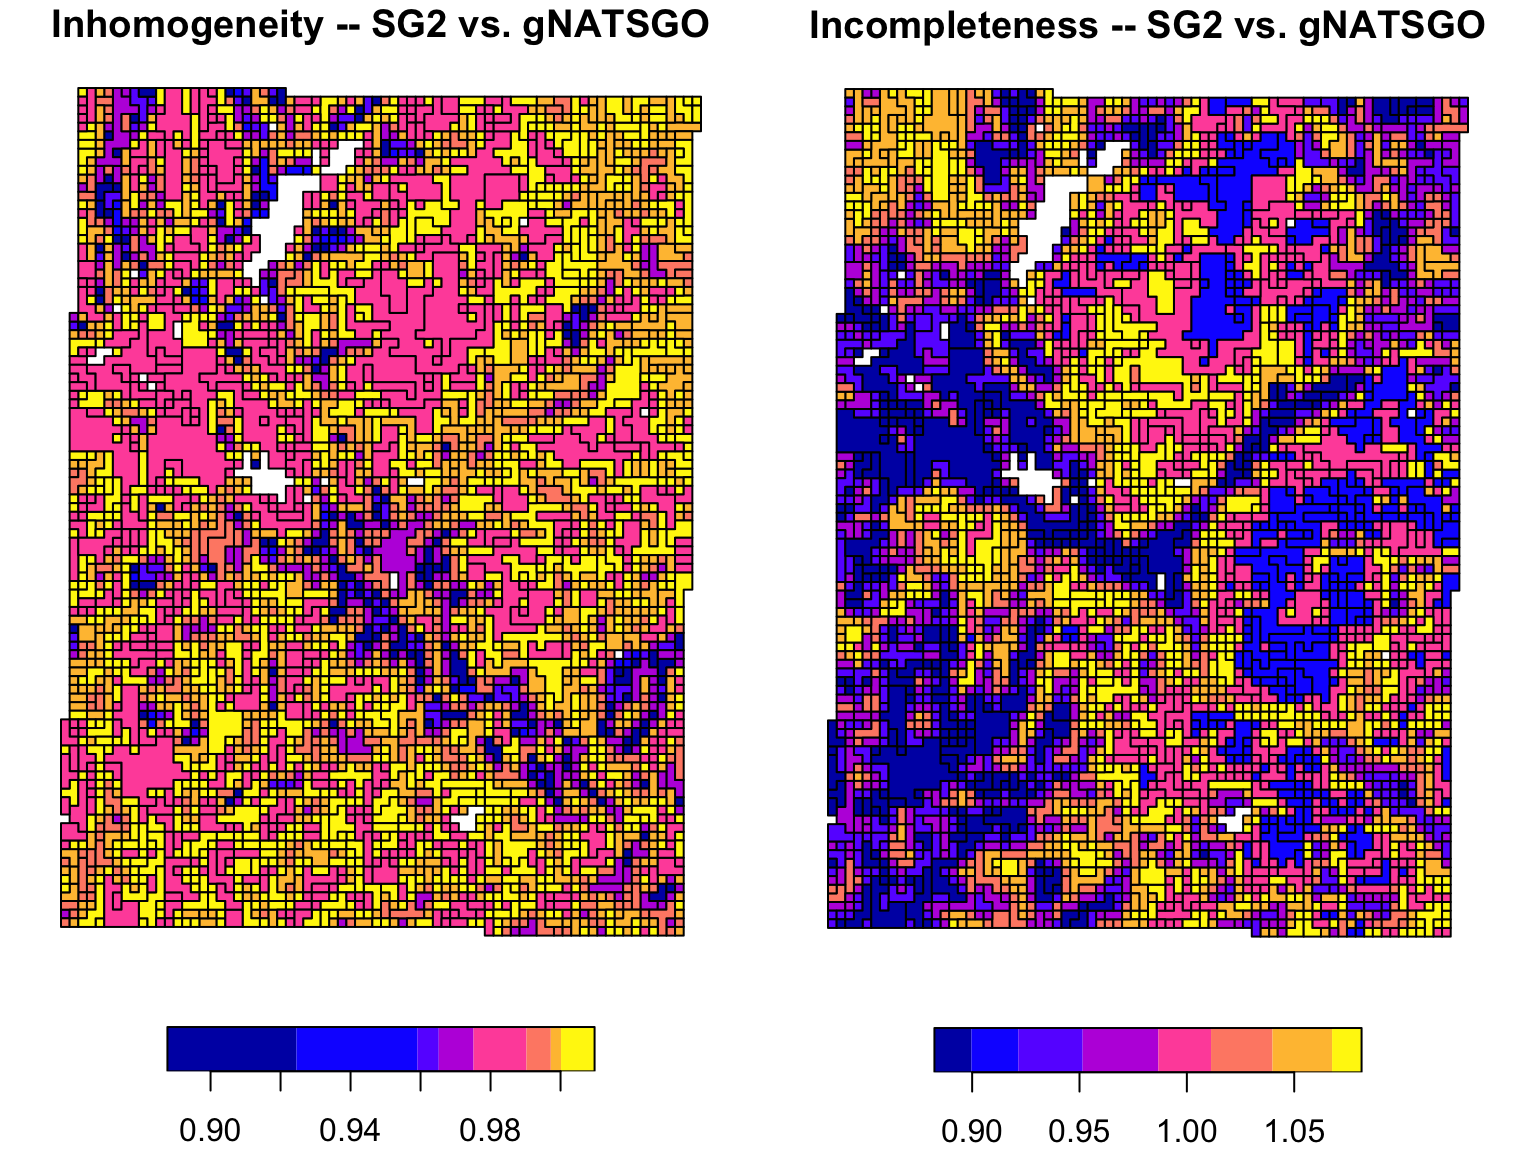
\includegraphics[height=0.72\textheight]{graphics_david/Fig16.png}
    \end{figure}
\end{frame}


\begin{frame}{V-measure example}
% latex table generated in R 4.1.2 by xtable 1.8-4 package
% 
\begin{tabular}{llll}
  \hline
DSM\hspace{1ex}products & V-measure & Homogeneity & Completeness \\ 
  \hline
gNATSGO vs.\ SG2 & 0.0128 & 0.0143 & 0.0116 \\ 
  gNATSGO vs.\ SPCG & 0.0258 & 0.0275 & 0.0243 \\ 
  gNATSGO vs.\ PSP & 0.084 & 0.0897 & 0.079 \\ 
  SPCG vs.\ SG2 & 0.3342 & 0.3495 & 0.3201 \\ 
   \hline
\end{tabular}
   
\par
V-measure statistics, pHx10 0--5~cm
\end{frame}

\begin{frame}{Metric: Co-occurrence vector}
  \begin{itemize}
  \item 
    Summarizes the entire \textbf{adjacency structure} of a map as a    normalized co-occurrence matrix: which classes are spatially adjacent to each other?
  \item
    This is a probability vector for the spatial co-occurrence of
    different    classes in the map.
    \item
    The ``distance'' between co-occurrence vectors from two maps can be computed   as a measure of the (dis)similarity between these structures
    (Jensen-Shannon distance, used to compare probability distributions)
  \end{itemize}
\end{frame}

\begin{frame}{Segmentation by patterns}
\begin{itemize}
    \item 
A recent development by Nowosad\footnote{https://jakubnowosad.com/}, based on an algorithm of Jadiewicz    
\item Aggregates groups of pixels (size set by analyst) into polygons with a ``similar enough'' spatial \textbf{pattern} of classes
\item The pattern of thse polygons could be considered a \textbf{meta-pattern} of the DSM product
\end{itemize}
\end{frame}

\newpage
%\begin{frame}{Segmentation by patterns}
    \begin{figure}
        \centering        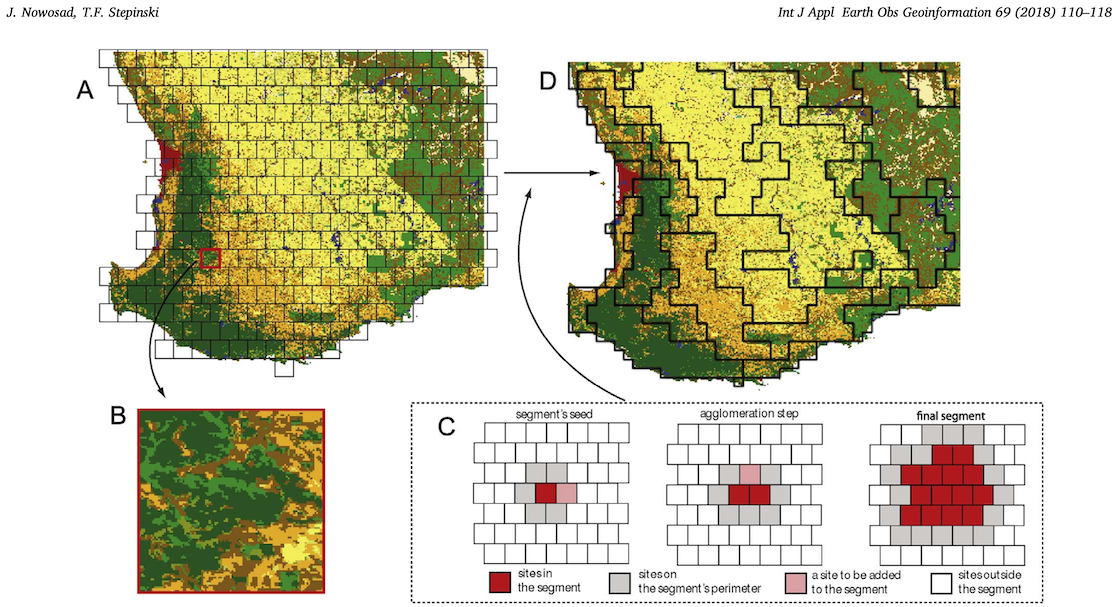
\includegraphics[height=0.9\textheight]{graphics_david/10.1016.j.jag.2018.03_Fig1.png}
    \end{figure}
%\end{frame}

\section{Comparing maps vs.\ ``reality''}

\begin{frame}{Comparing maps; maps vs.\ ``reality''}
    \begin{itemize}
        \item The pattern analysis applied to different maps can be compared
        \item The homogeneity and completeness of one map, representing the other, can be quantified
        \item The pattern of the \textbf{difference} map can be quantified
        \item But \ldots which is closest to the actual soil pattern \textbf{at the design scale}?
        \item Much knowledge from traditional soil survey about actual patterns at detailed mapping scales 1:12k -- 1:50k (Fridland 1974, Hole 1978)
    \end{itemize}
\end{frame}


\begin{frame}{Soil patterns as seen by traditional surveyors}
    \begin{figure}
        \centering
        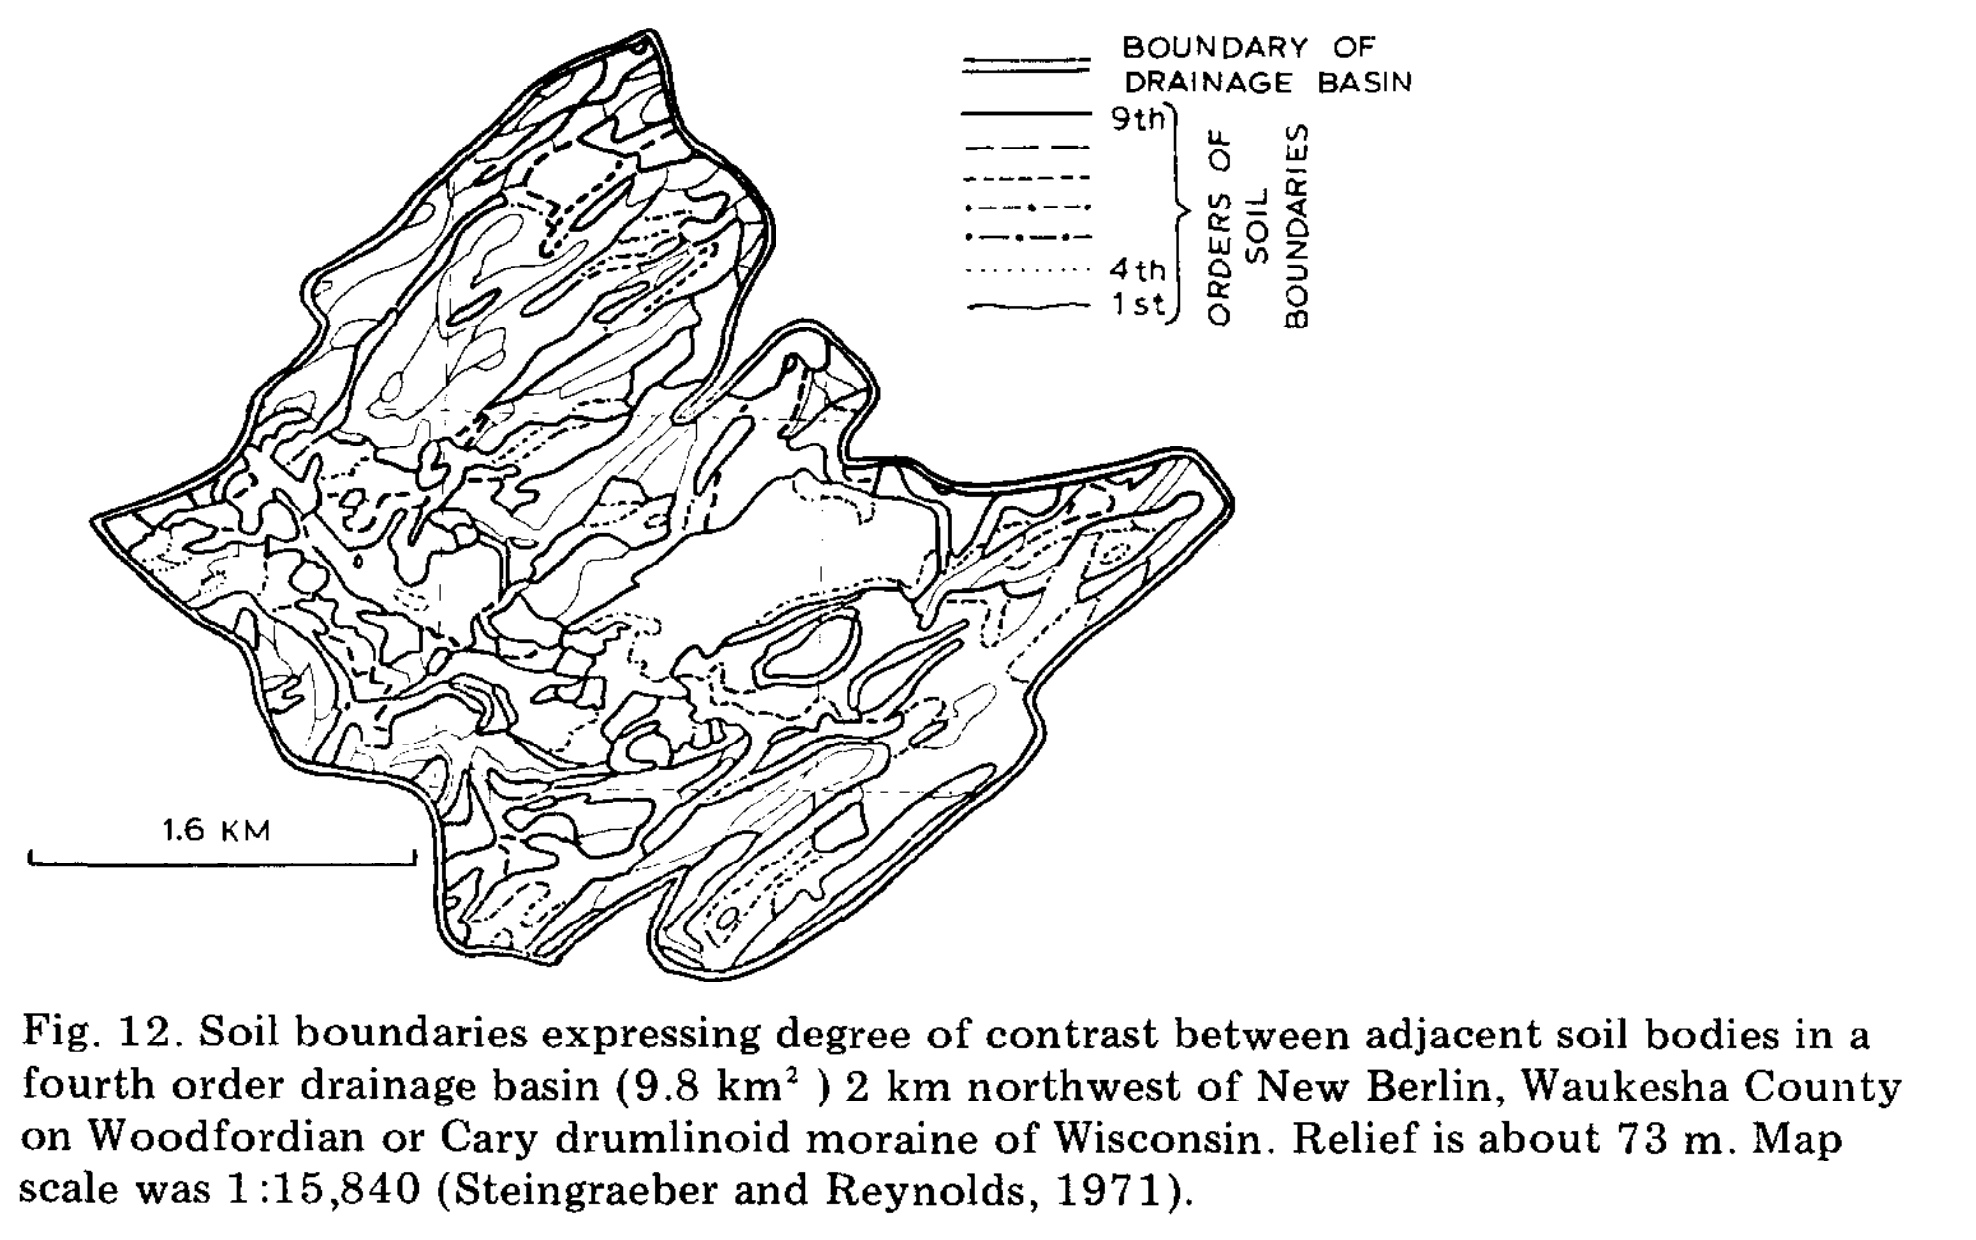
\includegraphics[height=0.75\textheight]{graphics_david/10.1016.0016-7061(78)90002-2_Fig12.png}
\\source: Hole (1978)
    \end{figure}
\end{frame}

\begin{frame}{Resolution and scale}
DSMaps are \textbf{gridded} at some horizontal \textbf{resolution} (``pixel size'') -- what is the relation to map scale?
\\[2ex]
    \begin{figure}
    \centering
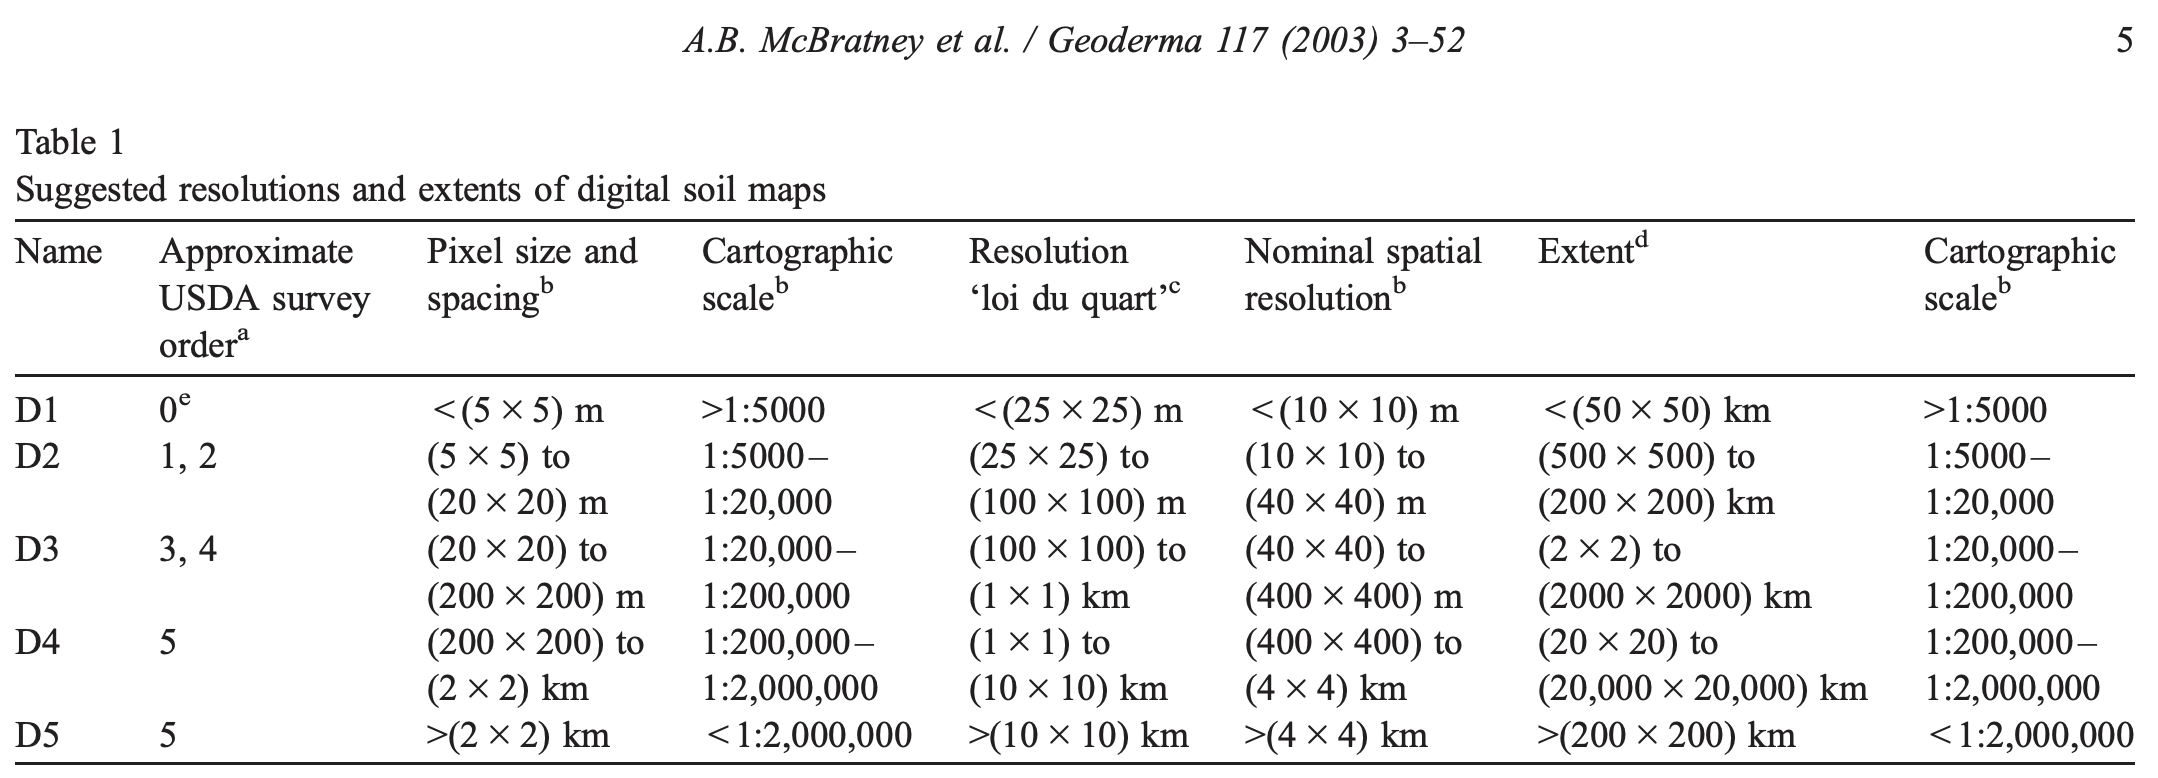
\includegraphics[width=\textwidth]{./graphics_david/McBratney2013_Table1.png}
\end{figure}
\end{frame}

\begin{frame}
  \frametitle{DSM scale effects -- 20 vs.\ 250~m resolution gSSURGO}
    \begin{figure}
    \centering
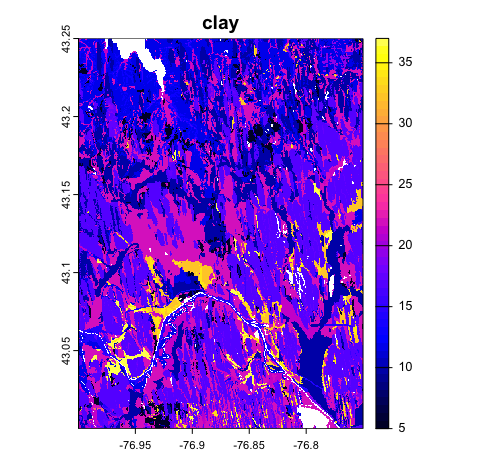
\includegraphics[width=0.45\textwidth]{./graphics_david/ClydeNY_gSSURGO_20.png}
\hfill
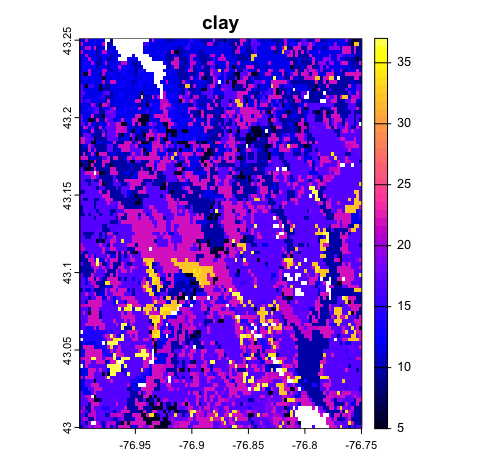
\includegraphics[width=0.45\textwidth]{./graphics_david/ClydeNY_gSSURGO_250.png}
\end{figure}  
\end{frame}

\begin{frame}{What will the map be used for?}
    \begin{itemize}
        \item This governs the selection of grid cell size.
        \item The soil variability \emph{within} the grid cell is ignored \ldots
        \begin{itemize}
            \item \ldots for the map user \ldots
            \item so, for the evaluator
        \end{itemize}
        \item The \textbf{single value} of the grid cell represents the value the user will put in their ``model''
        \item The \textbf{uncertainty} of the grid cell is the uncertainty \textbf{of that predicted value}, \emph{not} the variance within the grid cell.
    \end{itemize}
\end{frame}

\begin{frame}{Should the DSM match the polygon map?}
    \begin{itemize}
        \item Maybe DSM finds the ``inclusions'' within the map unit polygon
        \item This depends on the DSM resolution vs.\ minimum legible delineation (MLD) derived from the design scale
        \begin{itemize}
            \item $0.4~\mathrm{cm}^2$ on map $\to$ ground area
            \item e.g., 1:24k $\to$ MLD 2.3~ha; 1:12k $\to$ 0.576~ha
            \item If 4 pixels per MLD, pixel resolution 96~m (1:24k), 48~m (1:12k)
        \end{itemize}
        \item There is no way to check this spatially, but the proportion can be compared to estimates
    \end{itemize}
\end{frame}
\section{On, on!}

\begin{frame}{Next steps}
\begin{enumerate}
    \item Clarify concepts
    \item Match metrics with soil patterns at various scales
    \item Quantify match with ``actual'' soil pattern at various scales
    \item \textbf{Still quite some confusion\ldots}, must use the ``little grey cells''
\end{enumerate}
\end{frame}

%----------------
% Closing frame

\setbeamertemplate{background}{ 

\includegraphics[width=\paperwidth,height=\paperheight]
{background_end.png}}

{ \setbeamertemplate{footline}{} % no footer on title
\begin{frame} 
\frametitle{}
\framesubtitle{}

 \begin{center}
 \vspace{0.5cm}
 \textcolor{isric_yellow}{\Large{Questions, comments, suggestions?}}
 \end{center}
\textcolor{isric_yellow}{www: \url{https://www.css.cornell.edu/faculty/dgr2/index.html}}
\\ 
\textcolor{isric_yellow}{e-mail: \url{david.rossiter@isric.org}; \url{d.g.rossiter@cornell.edu}}
\end{frame} 
}

\setbeamertemplate{background}{

\includegraphics[width=\paperwidth,height=\paperheight]
{background_slides.png}}

\setbeamertemplate{footline}[eawag] % set footer

\begin{frame}[allowframebreaks]{References}


  \begin{scriptsize}
\begin{itemize}

  \item Bohn, M. P., \& Miller, B. A. (2024). Locally enhanced digital soil mapping in support of a bottom-up approach is more accurate than conventional soil mapping and top-down digital soil mapping. Geoderma, 442, 116781. \url{https://doi.org/10.1016/j.geoderma.2024.116781}

    \item Boulaine, J. (1982). Remarques sur quelques notions élémentaires de la pédologie”. Cahiers O.R.S.T.O.M., série Pédologie, 19(1), 29-41.

      \item Eymard, A., Richer-de-Forges, \ldots \& Arrouays, D. (2024). Exploring the untapped potential of hand-feel soil texture data for enhancing digital soil mapping: Revealing hidden spatial patterns from field observations. Geoderma, 441, 116769. \url{https://doi.org/10.1016/j.geoderma.2023.116769}

    
    \item Fridland, V. M. (1974). Structure of the soil mantle. Geoderma, 12, 35-42. \url{https://doi.org/10.1016/0016-7061(74)90036-6}

    \item Hole, F. D. (1978). An approach to landscape analysis with emphasis on soils. Geoderma, 21(1), 1-23. \url{https://doi.org/10.1016/0016-7061(78)90002-2}

    \item Hudson, B. D. (1992). The soil survey as paradigm-based science. Soil Science Society of America Journal, 56(3), 836-841. \url{https://doi.org/0.2136/sssaj1992.03615995005600030027x}


    \item Jasiewicz, J., Netzel, P., \& Stepinski, T. (2015). GeoPAT: A toolbox for pattern-based information retrieval from large geospatial databases. Computers \& Geosciences, 80, 62-73. \url{https://doi.org/10.1016/j.cageo.2015.04.002}


    \item Lagacherie, P., Andrieux, P., \& Bouzigues, R. (1996). Fuzziness and uncertainty of soil boundaries: From reality to coding in GIS. In P. A. Burrough, A. U. Frank, \& F. Salgé (Red.), Geographic objects with indeterminate boundaries (pp. 275-286). Taylor \& Francis.

    \item McBratney, A. B., Mendon\c{c}a Santos, M. L., \& Minasny, B. (2003). On digital soil mapping. Geoderma, 117(1-2), 3-52. \url{https://doi.org/10.1016/S0016-7061(03)00223-4}

    \item Nowosad, J. (2021). Motif: An open-source R tool for pattern-based spatial analysis. Landscape Ecology, 36(1), 29-43. \url{https://doi.org/10.1007/s10980-020-01135-0}

    
    \item Nowosad, J., \& Stepinski, T. F. (2018). Towards machine ecoregionalization of Earth’s landmass using pattern segmentation method. International Journal of Applied Earth Observation and Geoinformation, 69, 110-118. \url{https://doi.org/10.1016/j.jag.2018.03.004}

    \item Riitters, K. H., Vogt, P., Soille, P., Kozak, J., \& Estreguil, C. (2007). Neutral model analysis of landscape patterns from mathematical morphology. Landscape Ecology, 22(7), 1033-1043. \url{https://doi.org/10.1007/s10980-007-9089-3}

    \item Riitters, K., Vogt, P., Soille, P., \& Estreguil, C. (2009). Landscape patterns from mathematical morphology on maps with contagion. Landscape Ecology, 24(5), 699-709. \url{https://doi.org/10.1007/s10980-009-9344-x}

    \item Sciaini, M., Fritsch, M., Scherer, C., \& Simpkins, C. E. (2018). NLMR and landscapetools: An integrated environment for simulating and modifying neutral landscape models in R. Methods in Ecology and Evolution, 9(11), 2240-2248.\url{https://doi.org/10.1111/2041-210X.13076}


    \end{itemize}
        
  \end{scriptsize}

\end{frame}

%----------------
\end {document}
